\chapter{Aplicaciones informáticas}
\label{cap:aplicacion}

En este capítulo se describen las aplicaciones informáticas que se han desarrollado como complemento a las ideas que se exponen a lo largo del trabajo y que servirán de gran ayuda para visualizar los resultados que se exponen. \\

Se ha desarrollado una aplicación en Python con varias funcionalidades. La primera de ellas permite generar el coloreado de las funciones complejas en un disco de radio arbitrario mientras que la segunda permite extender una función $f: \partial \disk \to \complex$ apropiada a una función armónica en el disco abierto. Para producir el coloreado de ambas aplicaciones se utiliza la técnica de visualización de las funciones complejas conocida como coloreado del dominio. \\

\section{Técnica del coloreado del dominio}

En esta sección se presentan técnicas de visualización de las funciones complejas que permiten resaltar algunas propiedades analíticas o geométricas que poseen tales como la existencia de ceros y su multiplicidad, la de polos y su orden, la falta de continuidad, la periodicidad, etcétera. \\

A la hora de reflejar el comportamiento de funciones complejas, inmediatamente tenemos que lidiar con una dificultad implícita: los números complejos son bidimensionales, así que el grafo de una función $f : \complex \to \complex$, requerirá de cuatro dimensiones. La solución que propone \cite{Velleman2015} y que se va a emplear para representar estas funciones a lo largo del texto es la asignación de un color a cada número complejo. Esta forma de representación se denomina \textbf{Coloreado del dominio} (en inglés \textit{Domain Coloring}). \\

En concreto, la técnica del coloreado consiste en asignar a cada número complejo un determinado color que depende de su módulo y su argumento. La figura \ref{fig:z} muestra el plano complejo en el que a cada punto se le ha asignado un color distinto, de acuerdo al procedimiento que se describe a continuación. \\

En cuanto al argumento, conforme vamos aumentando el argumento el color recorre el círculo cromático, variando de rojo, amarillo, verde, cyan, azul, magenta y volviendo de nuevo al rojo. Según esta asignación, los puntos reales se corresponden con el rojo en el eje positivo mientras que en el eje negativo se corresponden con el cyan. \\

En lo que respecta al módulo, los puntos cercanos al origen se corresponden con colores oscuros mientras que los puntos alejados tienen colores claros. Así, cuando $\abs{z}$ tiende a $0$, el color asignado se acerca al negro, en cambio cuando $\abs{z}$ tiende a infinito, el color de $z$ se aproxima al blanco. \\

Con esta representación, cada número complejo tiene asignado un color diferente, por lo que un número complejo puede especificarse de manera única por su color. Dado $U \subset \complex$, podemos representar cualquier función $f: U \to \complex$ de la siguiente manera: a cada punto $z$ del dominio se le asigna el color correspondiente a $f(z)$. De este modo, se representa cualquier función compleja en dos dimensiones con los colores, tomando como referencia la figura \ref{fig:z}, que representa la función identidad $f(z) = z$ en el disco de radio $10$. \\

\begin{figure}[!htbp]
    \centering
    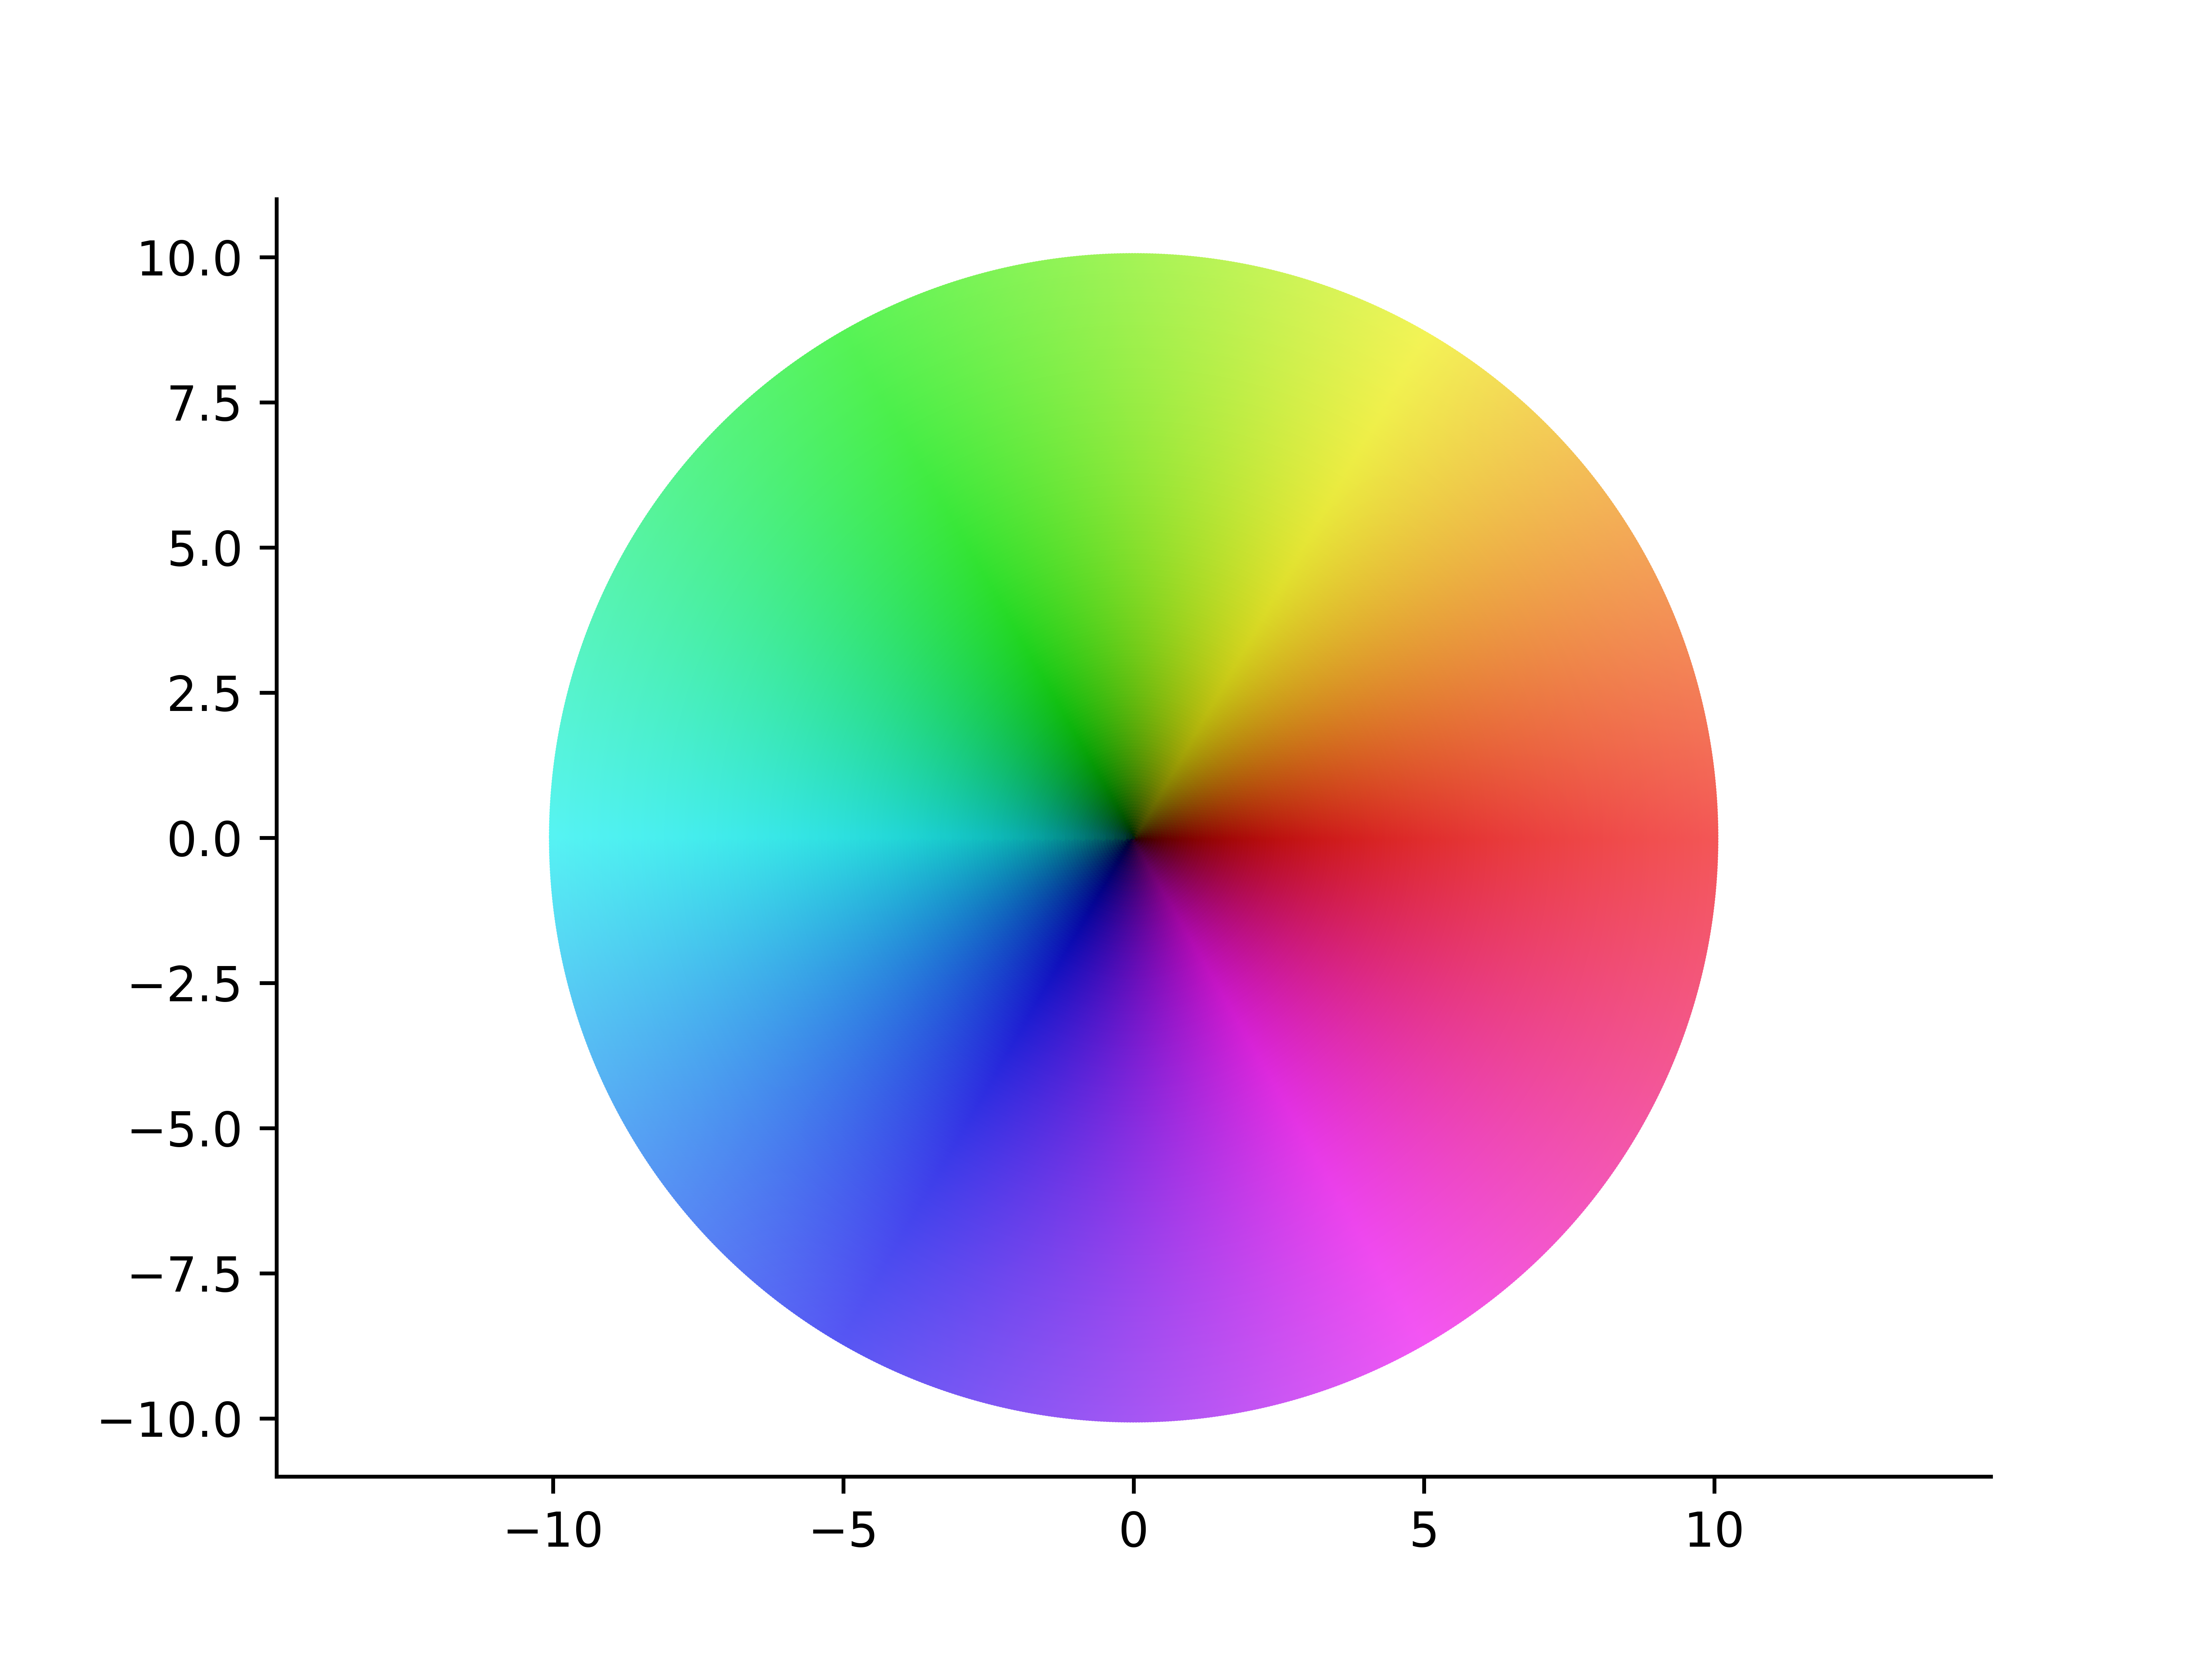
\includegraphics[width=0.7\textwidth]{../Aplicacion/z.png}
    \caption{Plano complejo coloreado}
    \label{fig:z}
\end{figure}

A continuación mostramos con unos ejemplos la gran cantidad de información que podemos extraer gracias a la representación de funciones complejas mediante la técnica de coloreado del dominio. \\

Por ejemplo, la figura \ref{fig:z^3} representa la función $f(z) = z^3$. Podemos observar que el centro del dibujo tiene un color muy oscuro. La razón es que cuando $\abs{z}$ es pequeño, $\abs{z^3}$ lo es mucho más, y por lo tanto el color asignado a $z^3$ es muy oscuro. También podemos ver que los colores se vuelven muy claros conforme nos vamos alejando del centro. Esto ocurre porque cuando $z$ es de módulo grande, también lo es $z^3$, y por consiguiente el color correspondiente es muy claro. \\

\begin{figure}[!htbp]
    \centering
    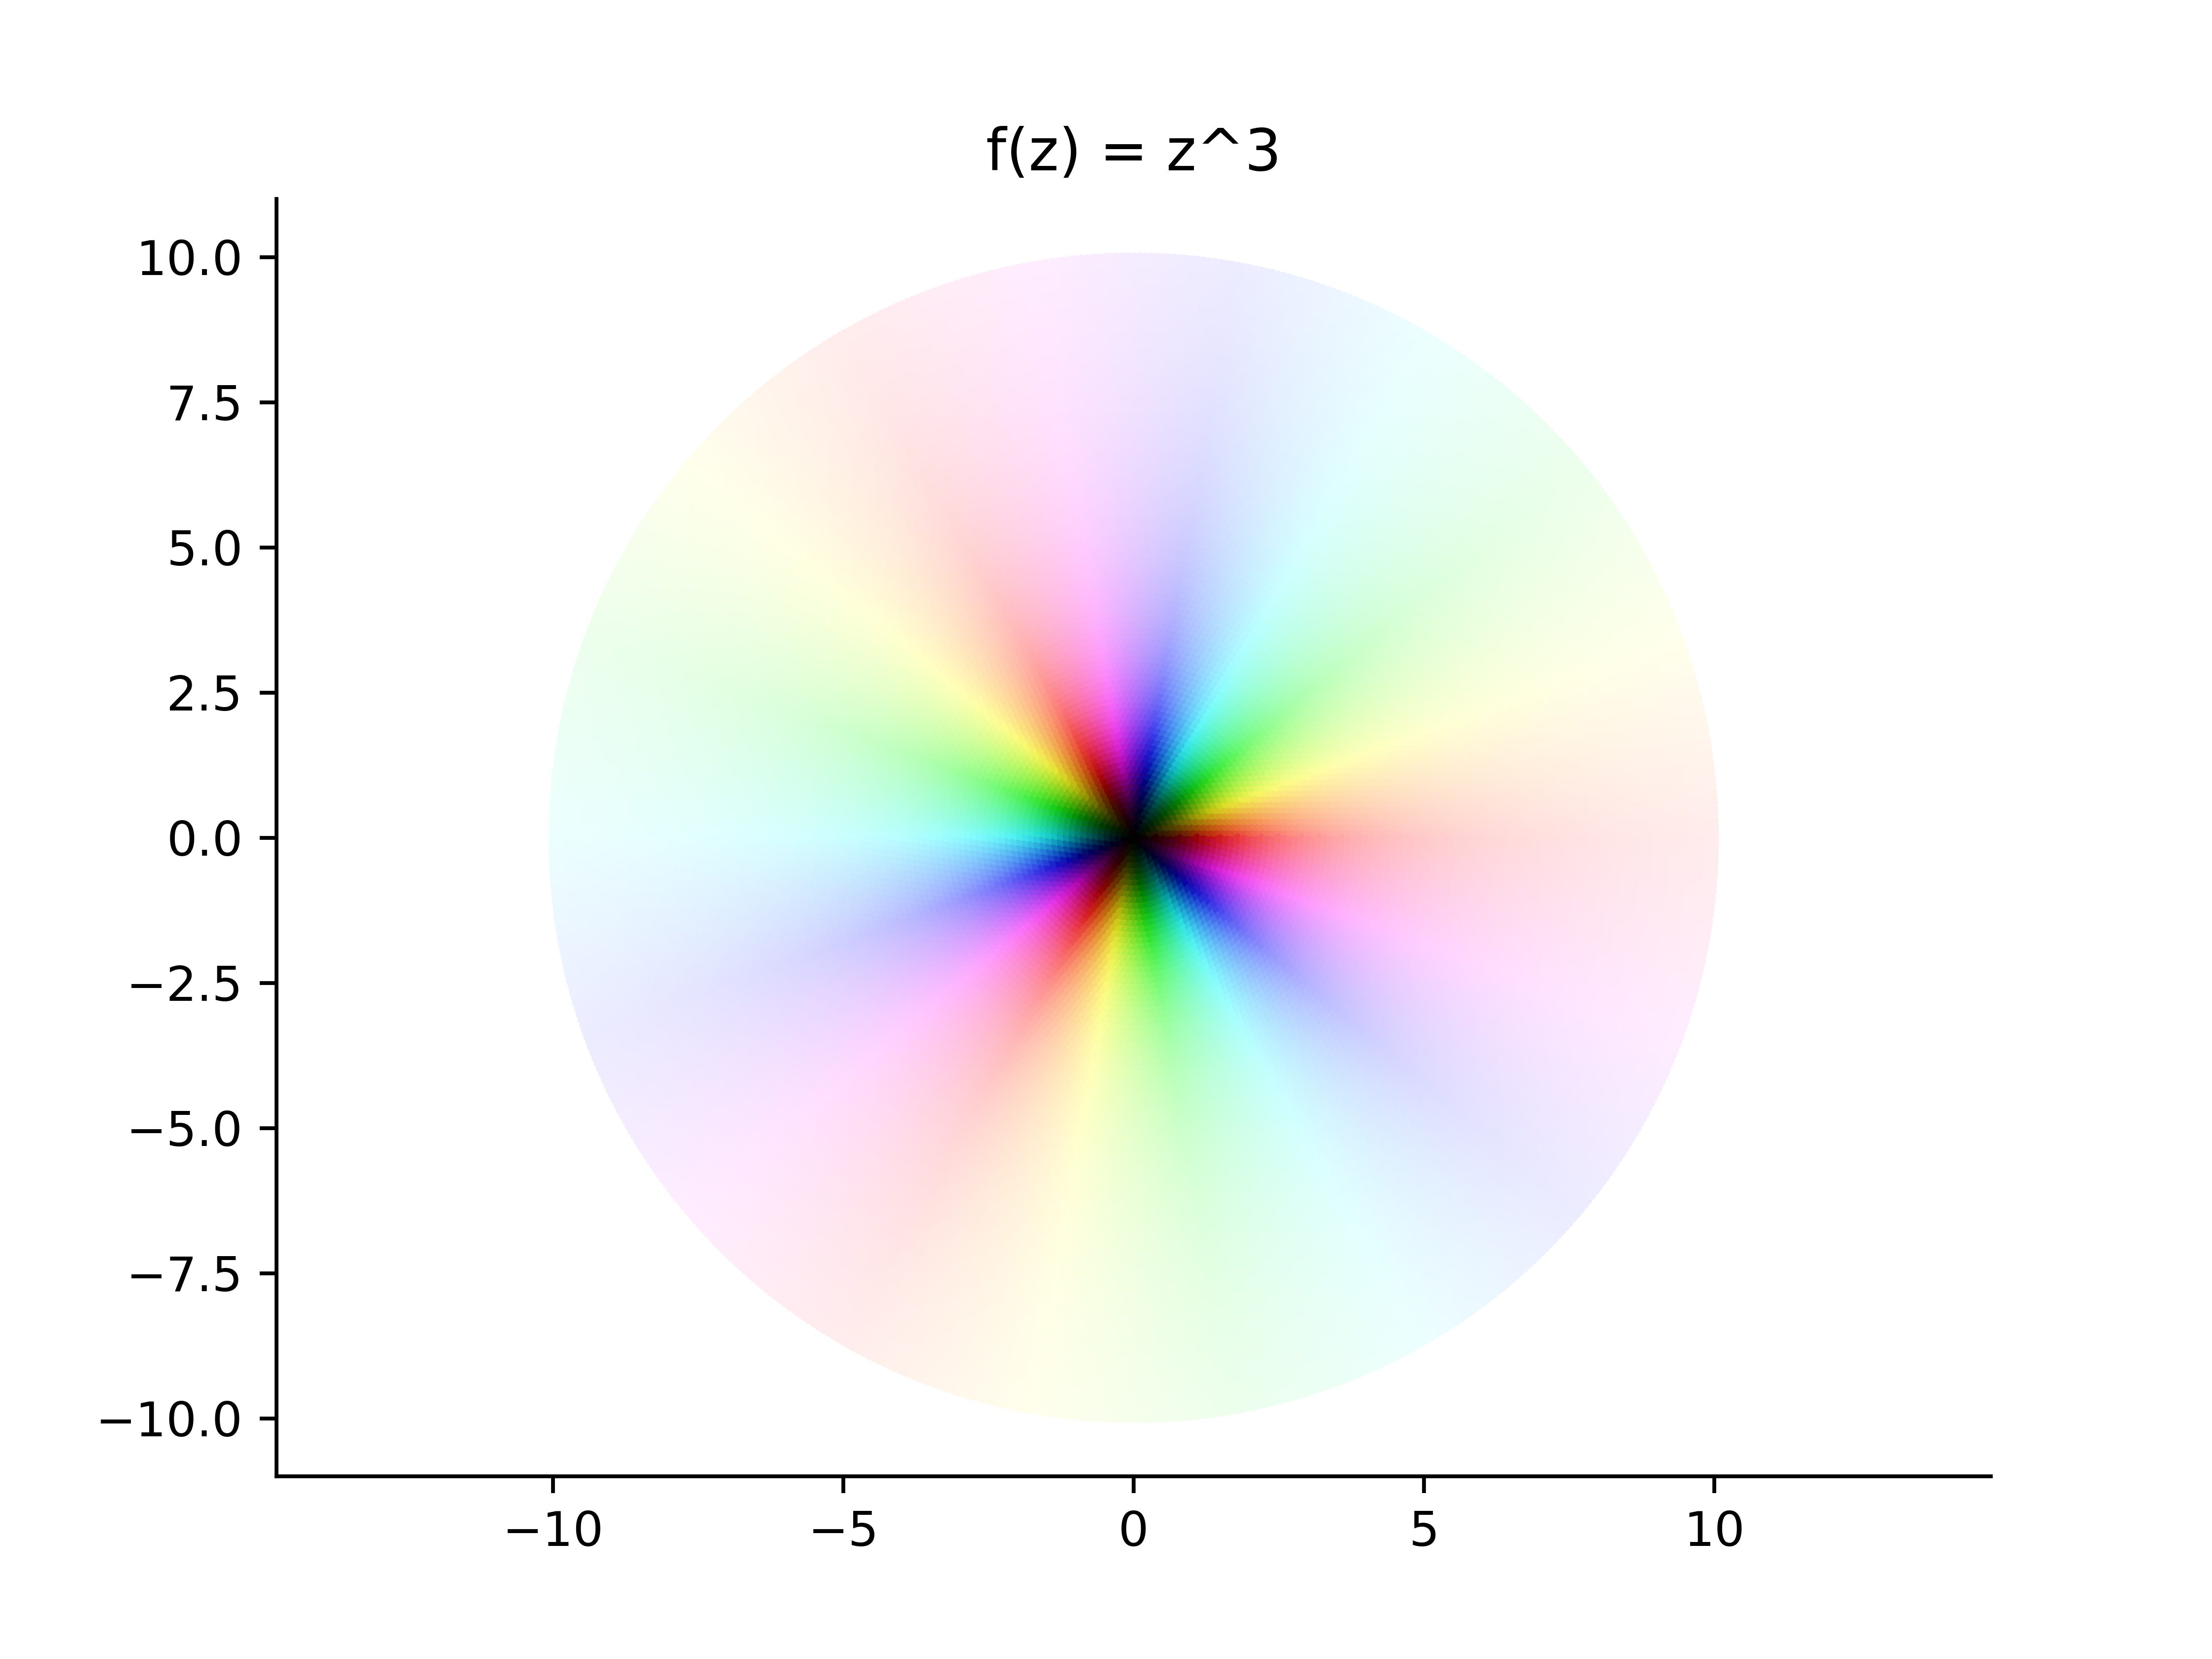
\includegraphics[width=0.7\textwidth]{../Aplicacion/z^3.png}
    \caption{Representación de la función $f(z) = z^3$.}
    \label{fig:z^3}
\end{figure}

Puesto que el color asignado al número $0$ es el negro, sabemos que las raíces del polinomio se corresponden con los puntos negros. En el caso que nos ocupa, el $0$ es una raíz triple de la función y se puede observar en que los colores del círculo cromático la envuelven tres veces. \\

Por último cuando avanzamos en el sentido contrario a las agujas del reloj, pasamos por los colores del círculo cromático $3$ veces. Esto muestra el hecho de que el argumento de $z^3$ es tres veces el argumento de $z$, y por lo tanto la imagen de un círculo centrado en el origen bajo la función cúbica se envuelve alrededor del origen tres veces. Esto se explica porque para cada número de módulo $s=r^3$ encontramos tres raíces distintas de módulo $r$. Si representamos la función $f(z)=e^{z^3}-1$, observamos una imagen que, cerca del $0$, es análoga a la anterior, pues tiene un cero triple en $z=0$. La figura \ref{fig:e^(z^3)-1} muestra este último ejemplo. \\

\begin{figure}[!htbp]
    \centering
    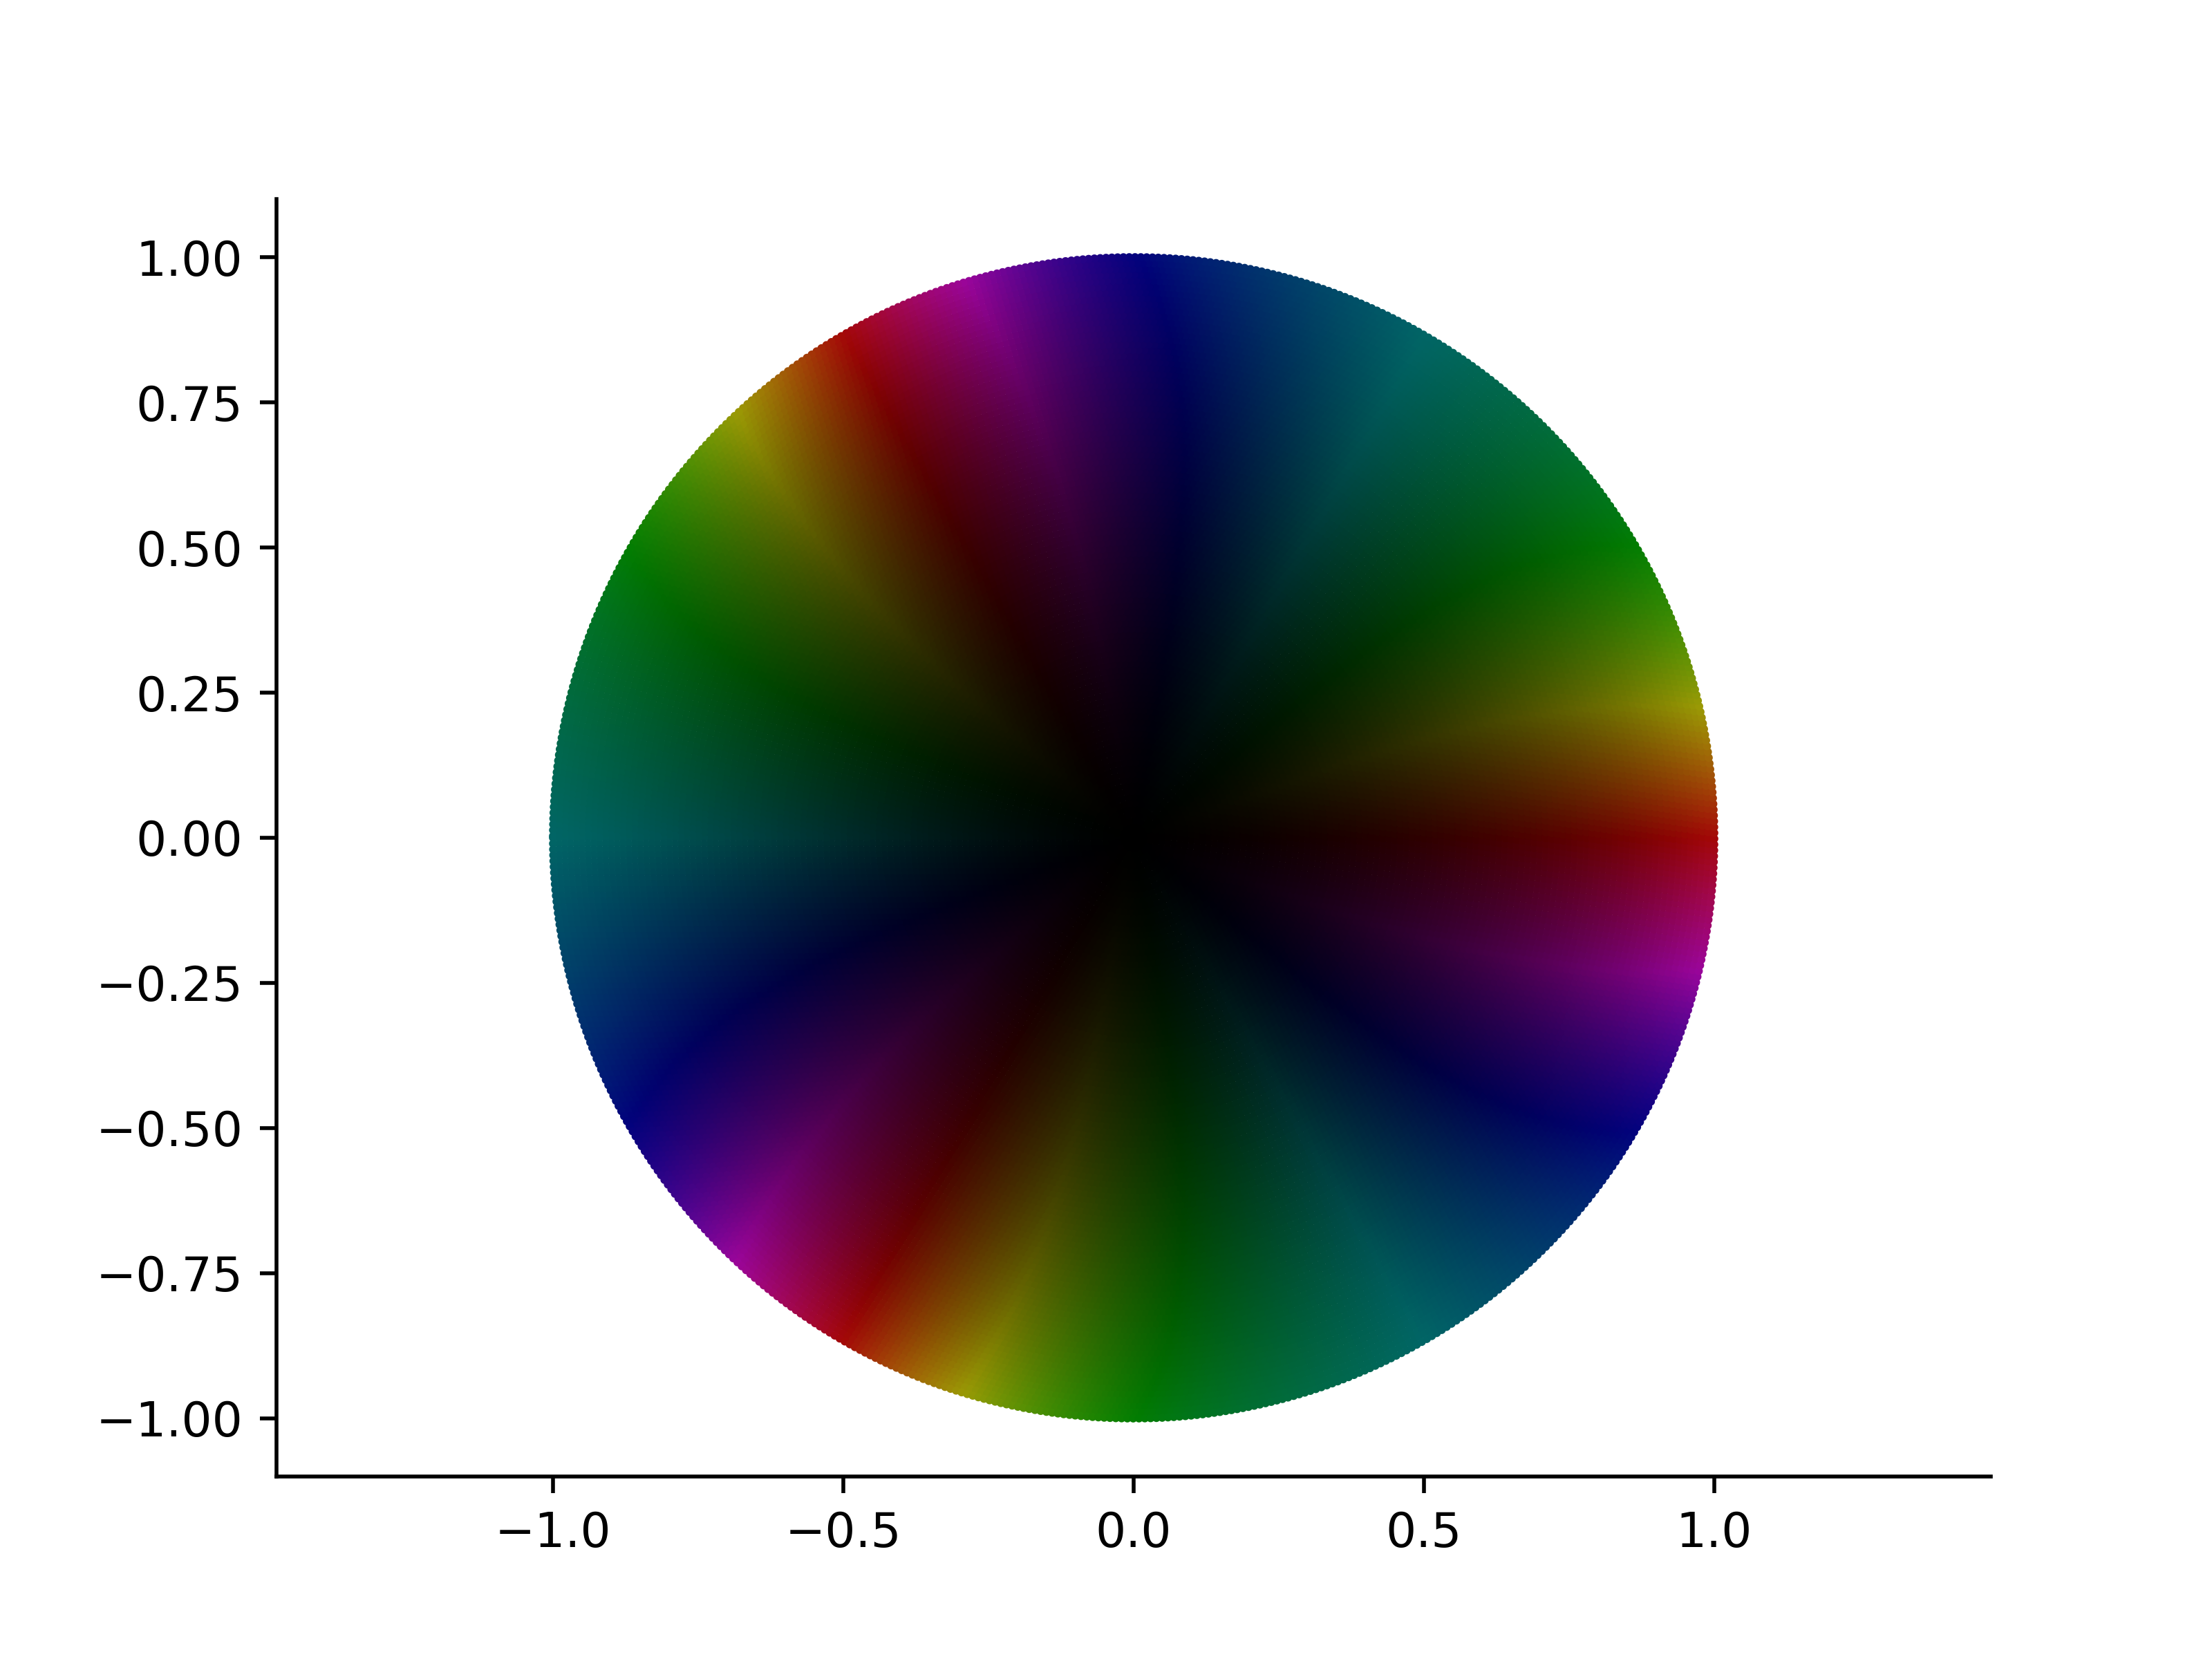
\includegraphics[width=0.7\textwidth]{../Aplicacion/e^(z^3)-1.png}
    \caption{Representación de la función $f(z) = e^{z^3}-1$.}
    \label{fig:e^(z^3)-1}
\end{figure}

La figura \ref{fig:1/z} muestra la representación de la función $f(z) = \frac{1}{z}$ con la técnica del coloreado. En este caso, el color que se le ha asignado al $0$ es blanco, lo que indica que $\frac{1}{z}$ tiende a infinito cuando $z$ tiende a $0$. Es decir, nos encontramos ante un polo de la función. Podemos observar que en el origen se envuelven los colores del círculo cromático una única vez en sentido contrario, lo que indica que se trata de un polo simple. La función $\frac{\cos z}{z}$, por ejemplo, también tiene un cero simple en $z=0$ y un representación análoga a $\frac{1}{z}$ en un entorno del origen. \\

\begin{figure}[!htbp]
    \centering
    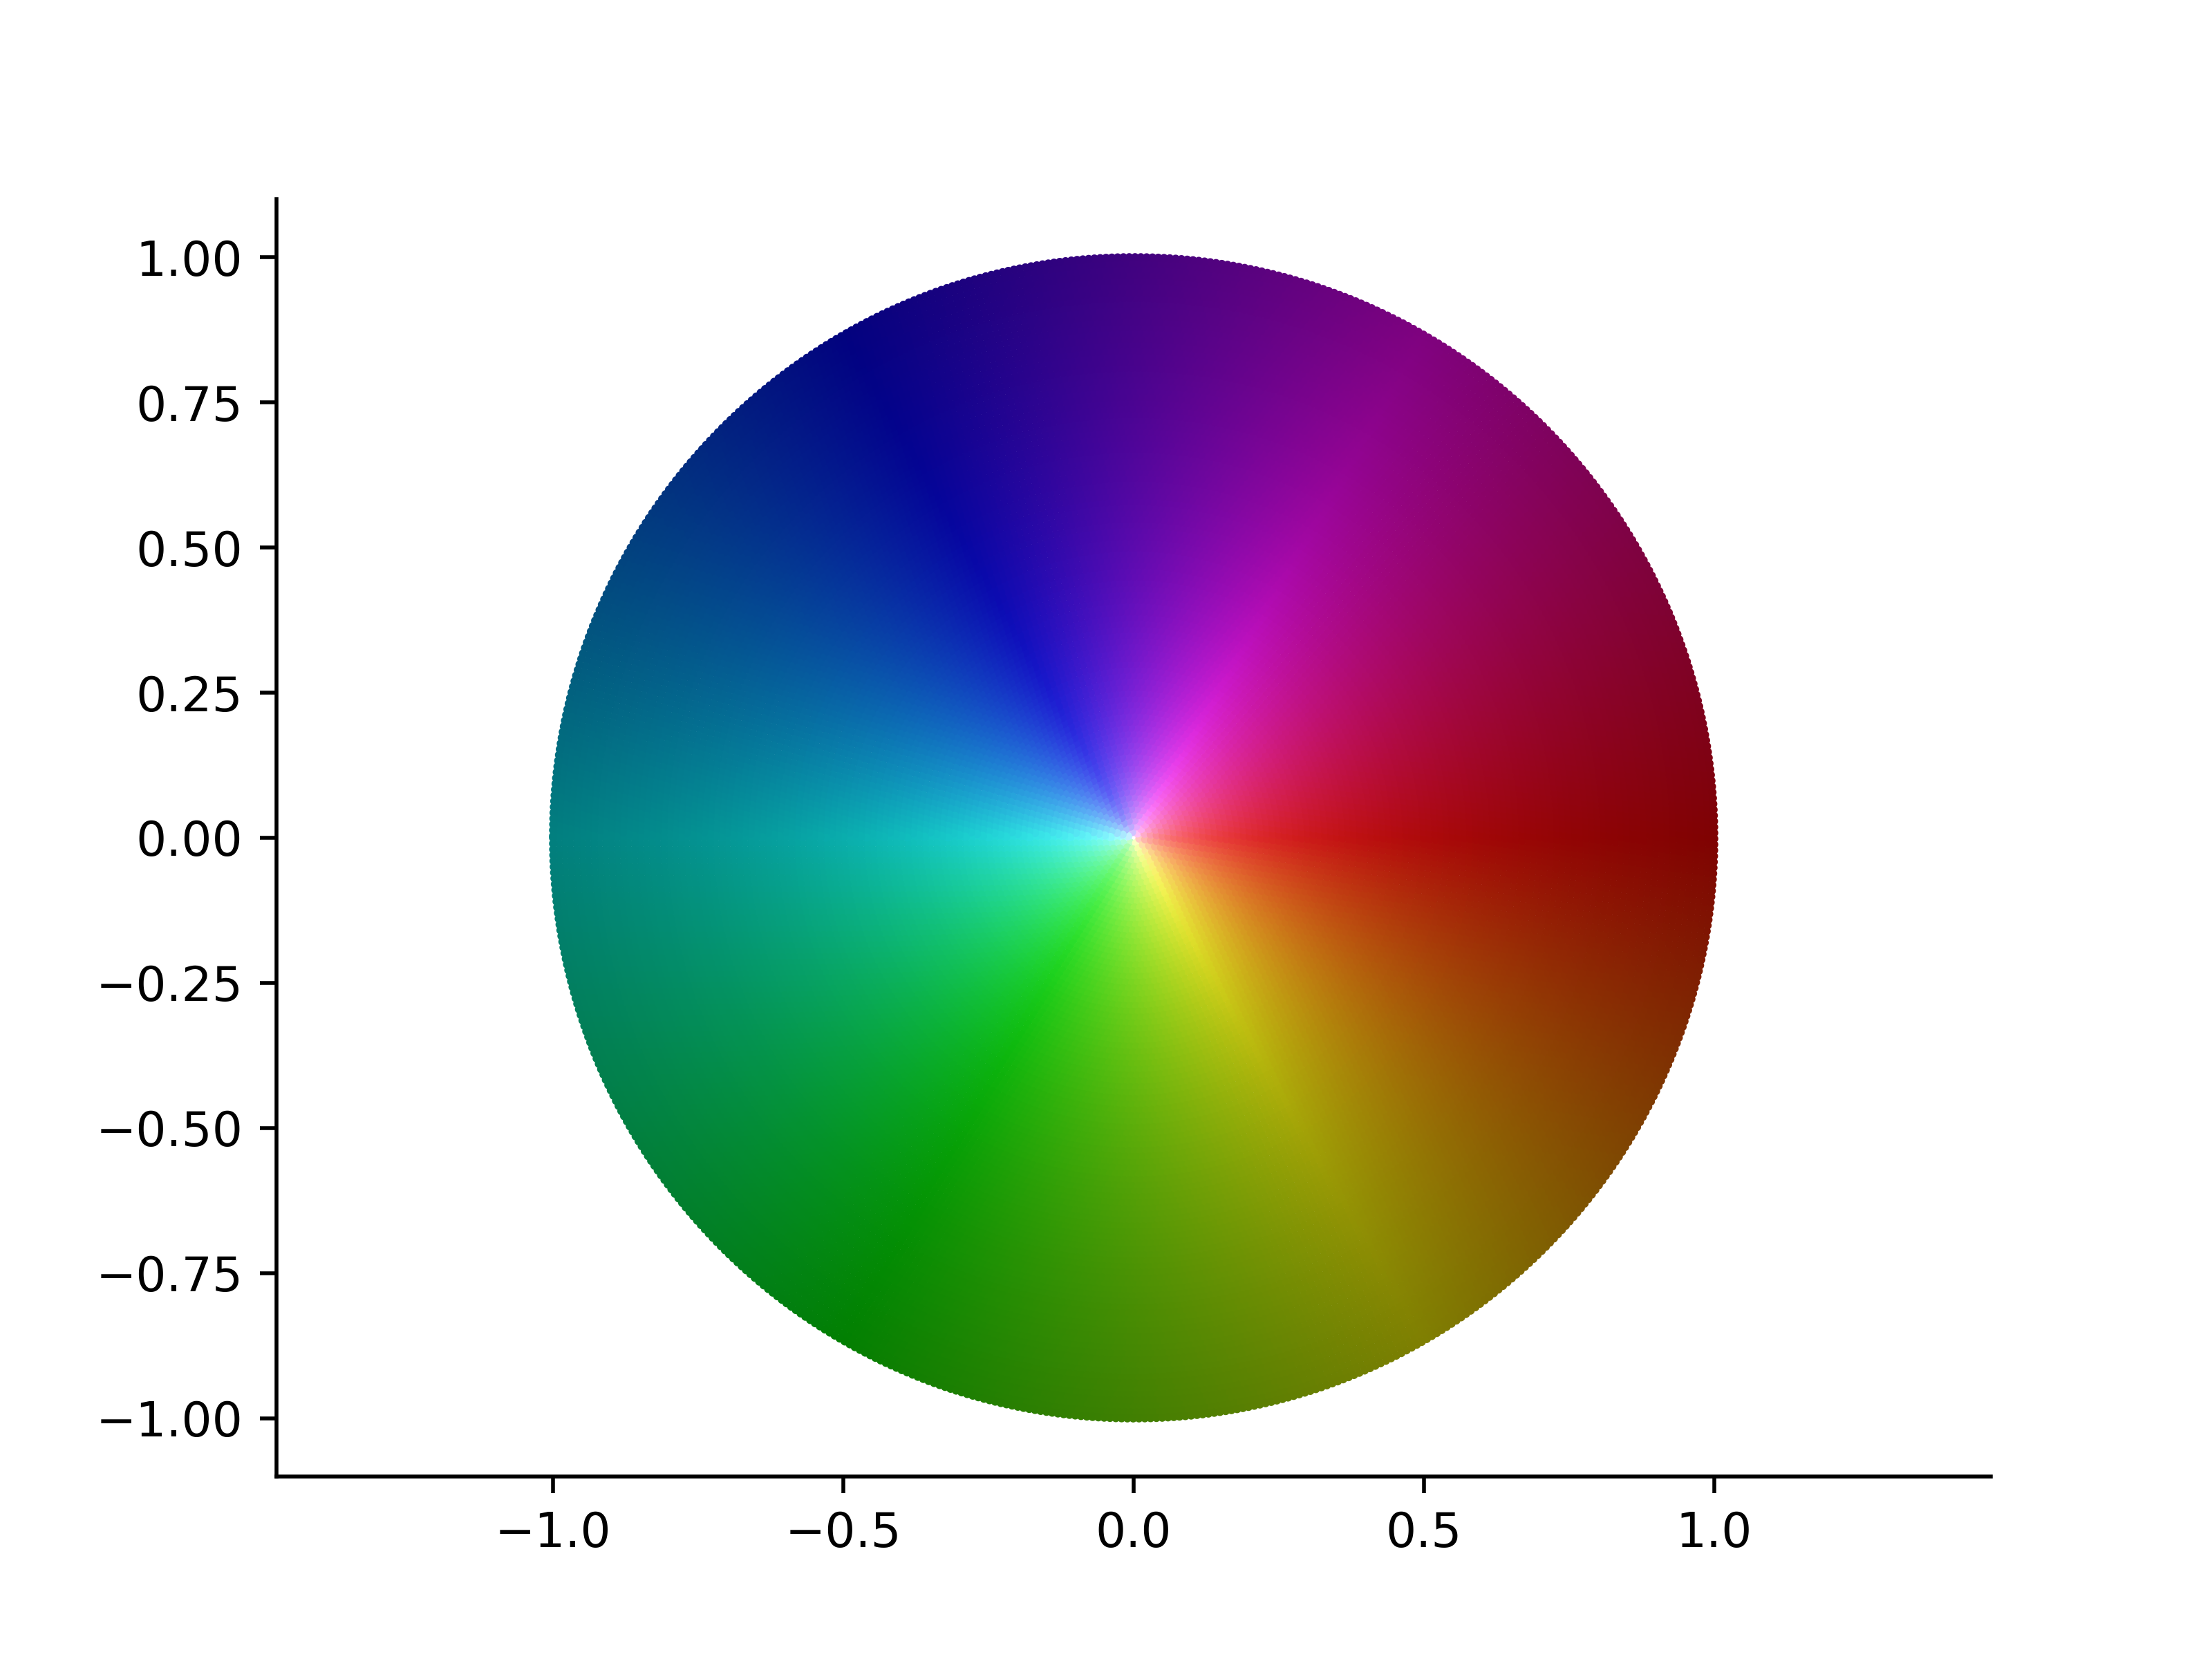
\includegraphics[width=0.7\textwidth]{../Aplicacion/1:z.png}
    \caption{Representación de la función $f(z) = \frac{1}{z}$.}
    \label{fig:1/z}
\end{figure}

Las funciones $e^z$ y $\sen(z)$ van a ilustrar el caso de las funciones periódicas. Se puede ver su representación en las figuras \ref{fig:e^z} y \ref{fig:sen(z)}, respectivamente. Observamos que en el caso de la exponencial ahora los colores van cambiando conforme avanzamos verticalmente. Si escribimos $z = x + iy$, entonces $e^z = e^{x+i y} = e^x e^{i y}$. Por lo que $y$, la parte imaginaria de $z$, determina el argumento y, por tanto, el color. Queda claro que el argumento es periódico de período $2 \pi$ en la dirección imaginaria. \\

\begin{figure}[!htbp]
    \centering
    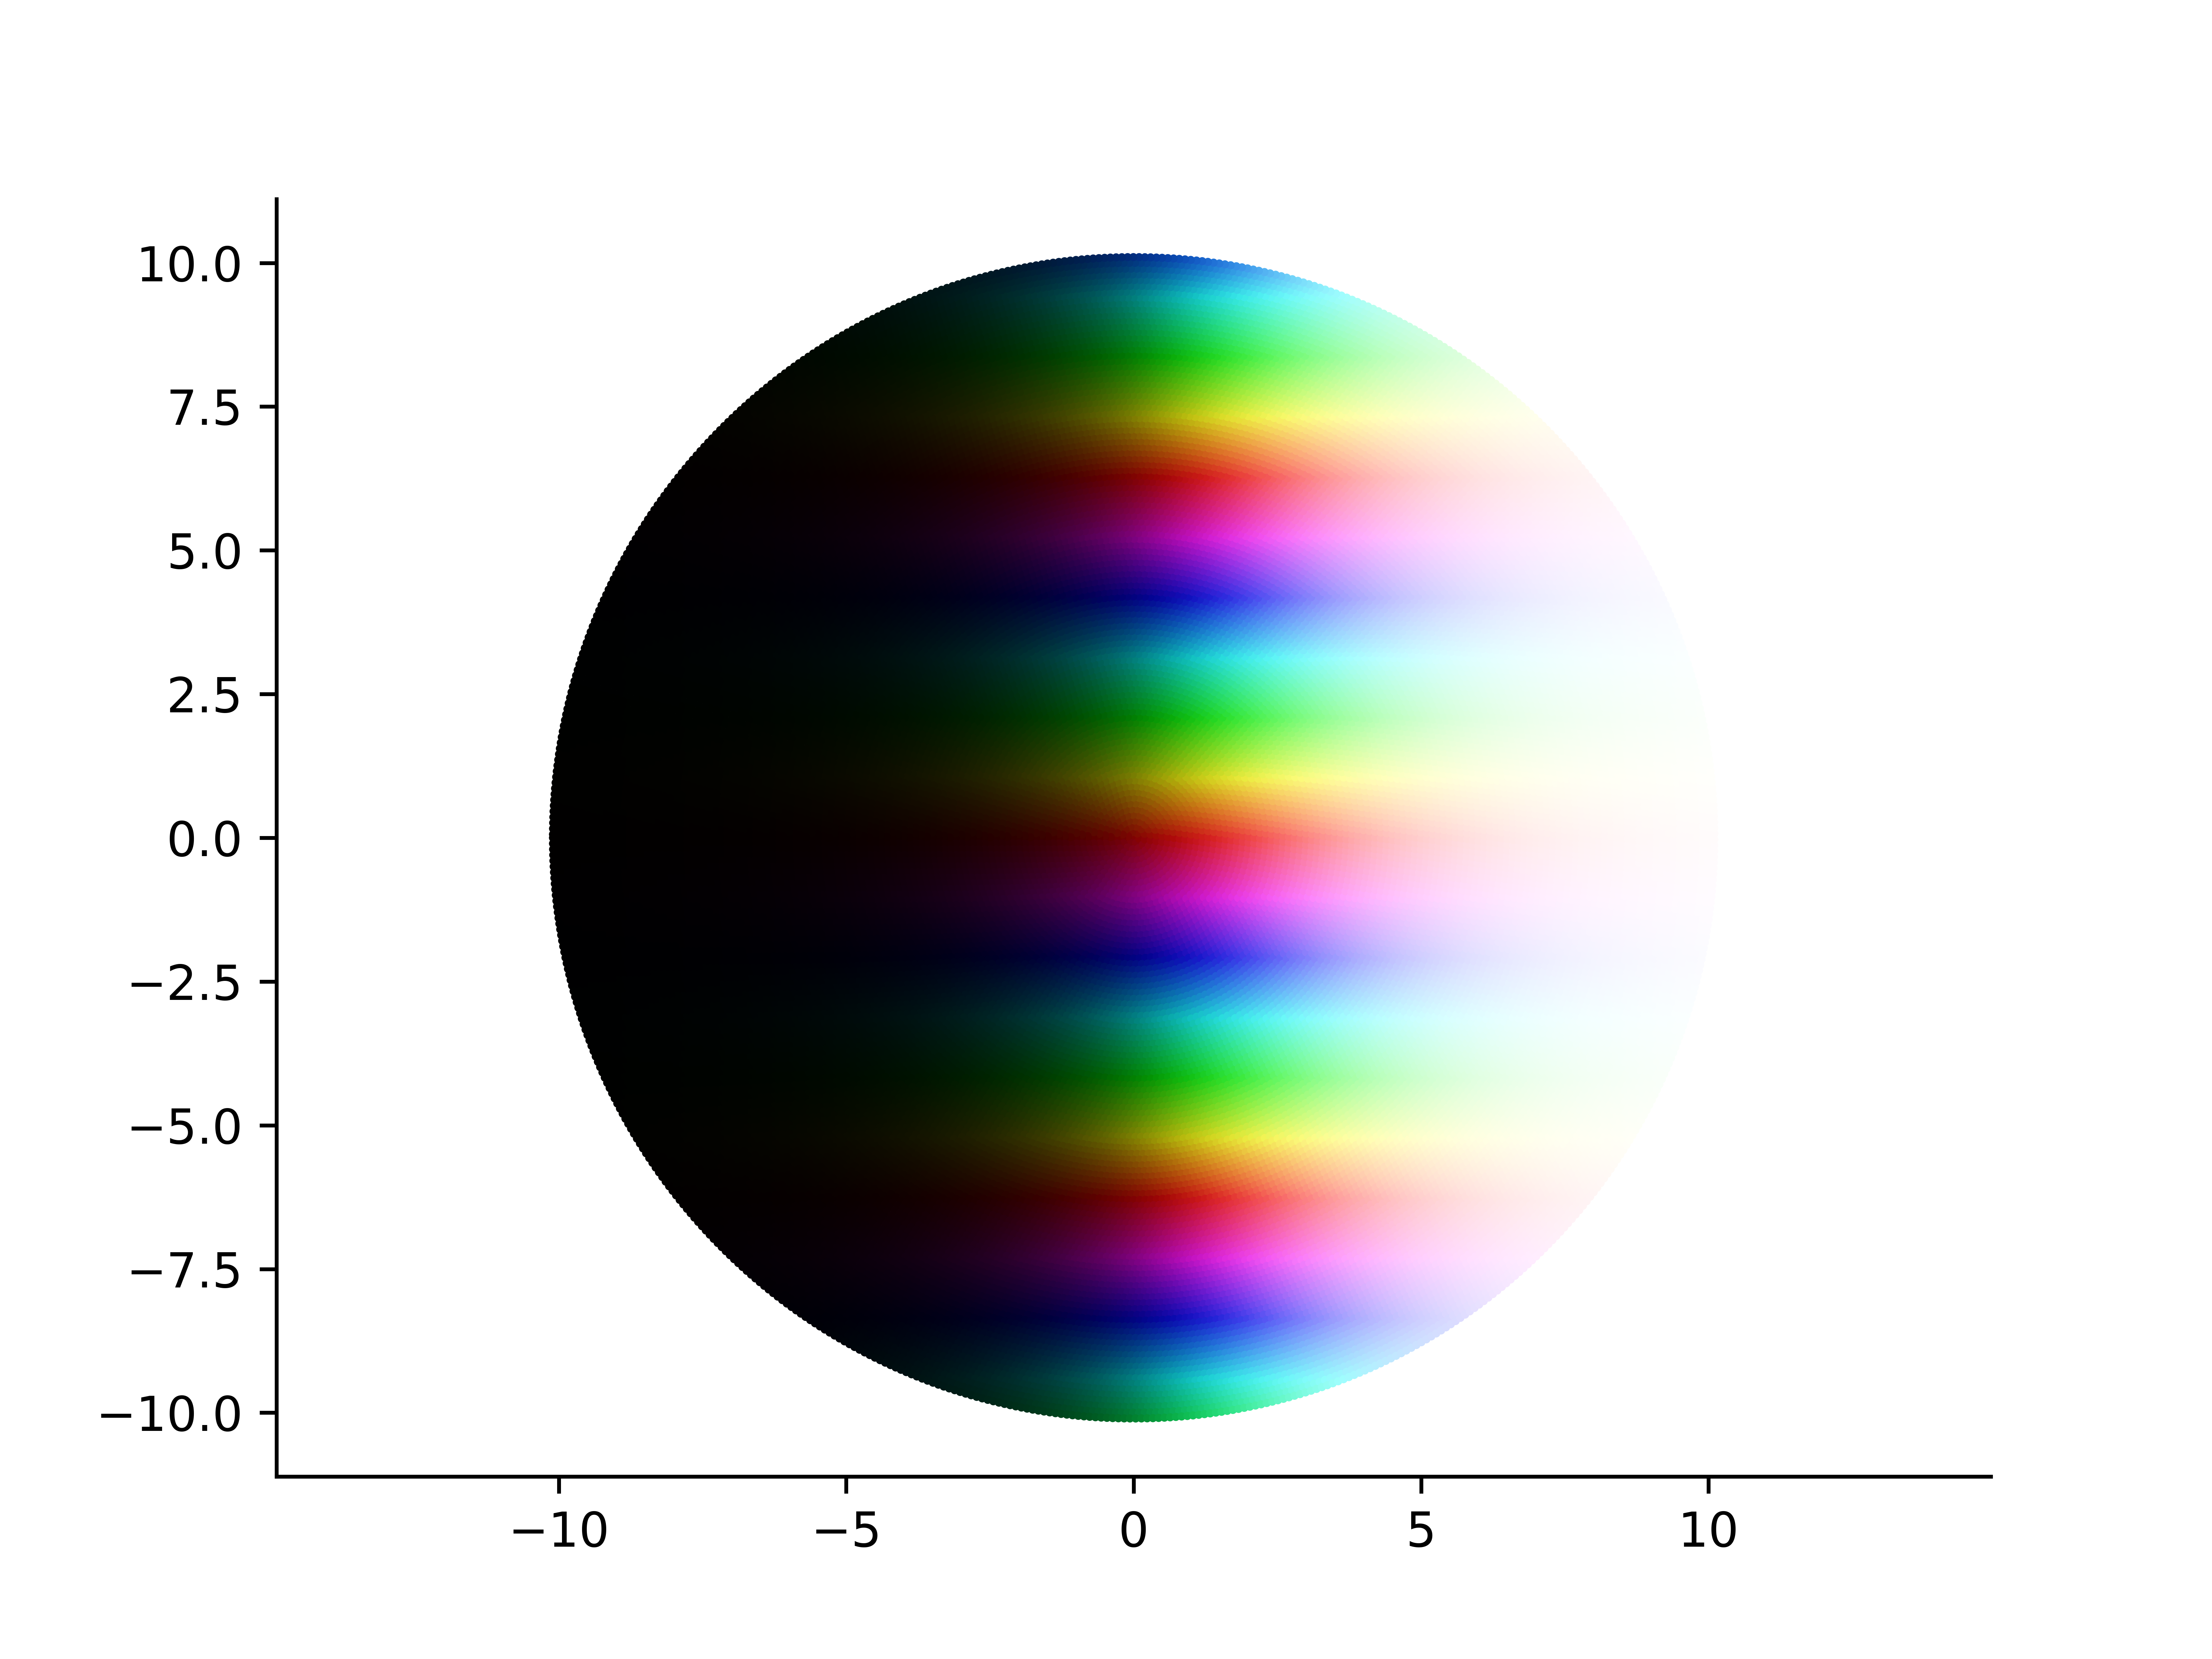
\includegraphics[width=0.7\textwidth]{../Aplicacion/e^z.png}
    \caption{Representación de la función $f(z) = e^z$.}
    \label{fig:e^z}
\end{figure}

\begin{figure}[!htbp]
    \centering
    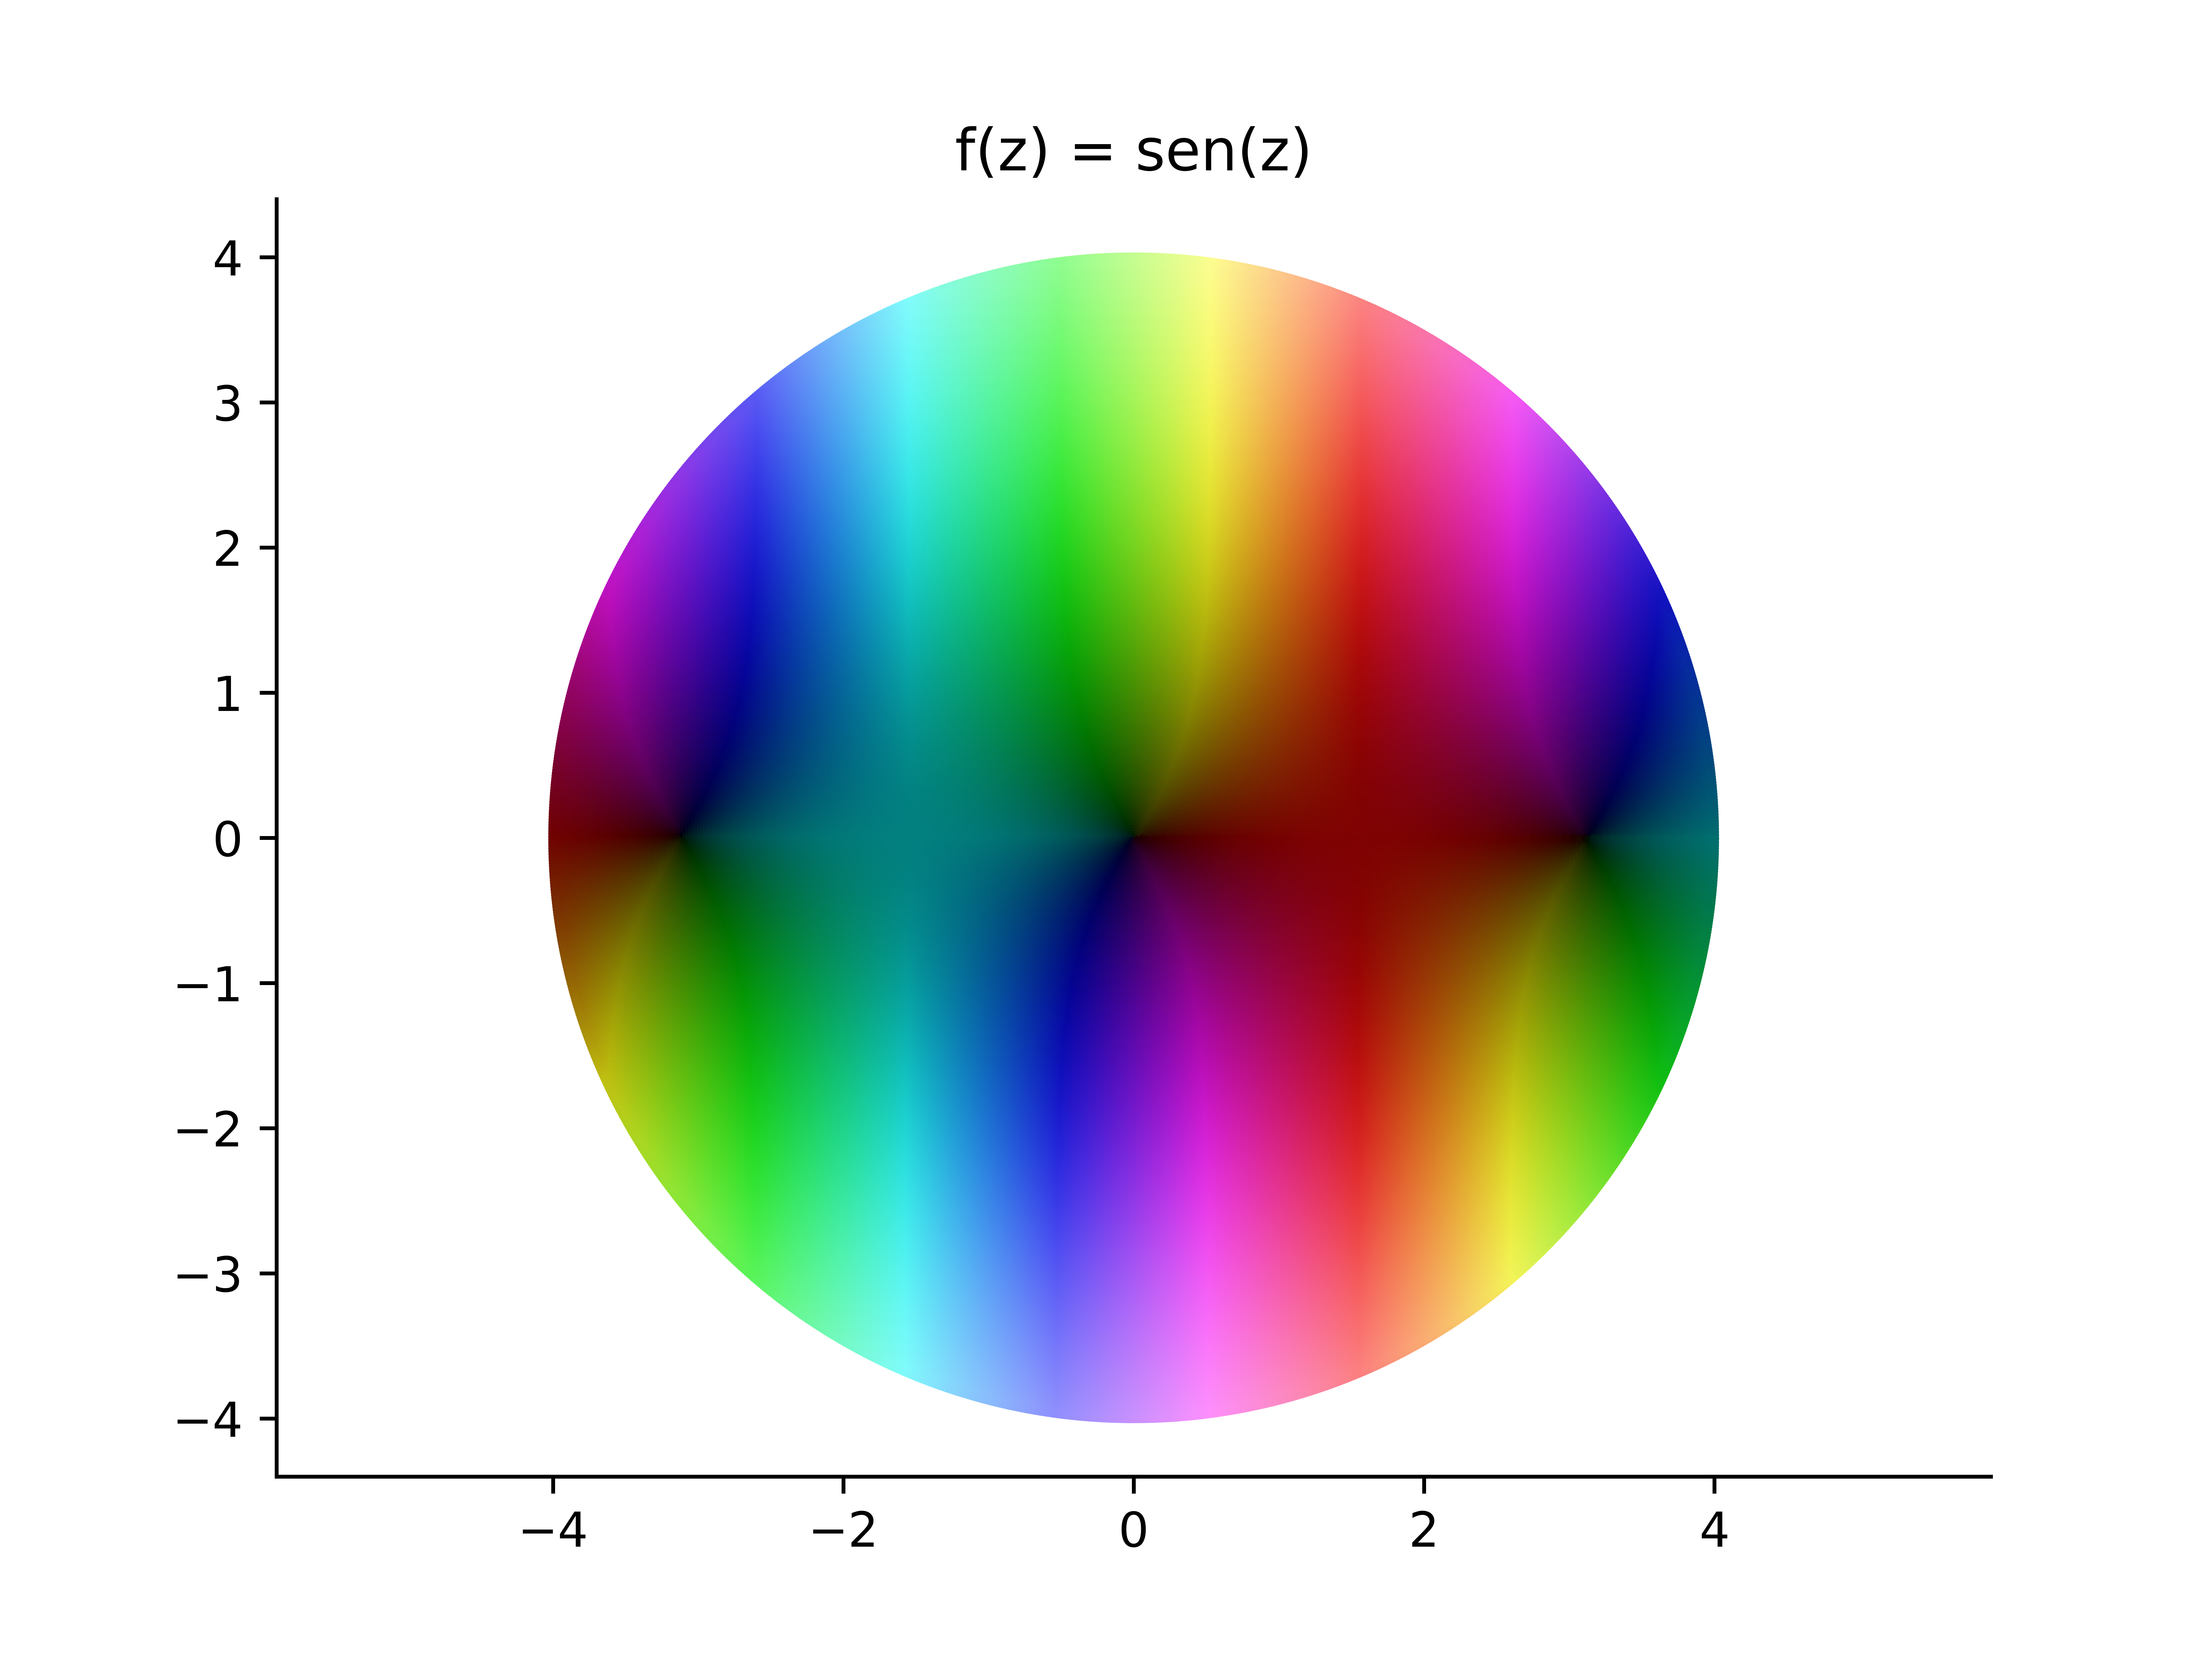
\includegraphics[width=0.7\textwidth]{../Aplicacion/sen(z).png}
    \caption{Representación de la función $f(z) = \sen(z)$.}
    \label{fig:sen(z)}
\end{figure}

La figura \ref{fig:log(z)} representa la función $\log(z)$, una función no continua. Al haber discontinuidad en una semirrecta -porque no se puede definir un argumento continuo-, queda muy patente que la técnica del coloreado permite detectar estas discontinuidades. También es muy drástico cómo se ven las singularidades esenciales, por ejemplo, en $z = 0$ para $\sen(\frac{1}{z})$. En el capítulo \ref{cap:ejemplos} se mostrará mediante un ejemplo cómo se representan las singularidades esenciales con la técnica del coloreado. \\

\begin{figure}[!htbp]
    \centering
    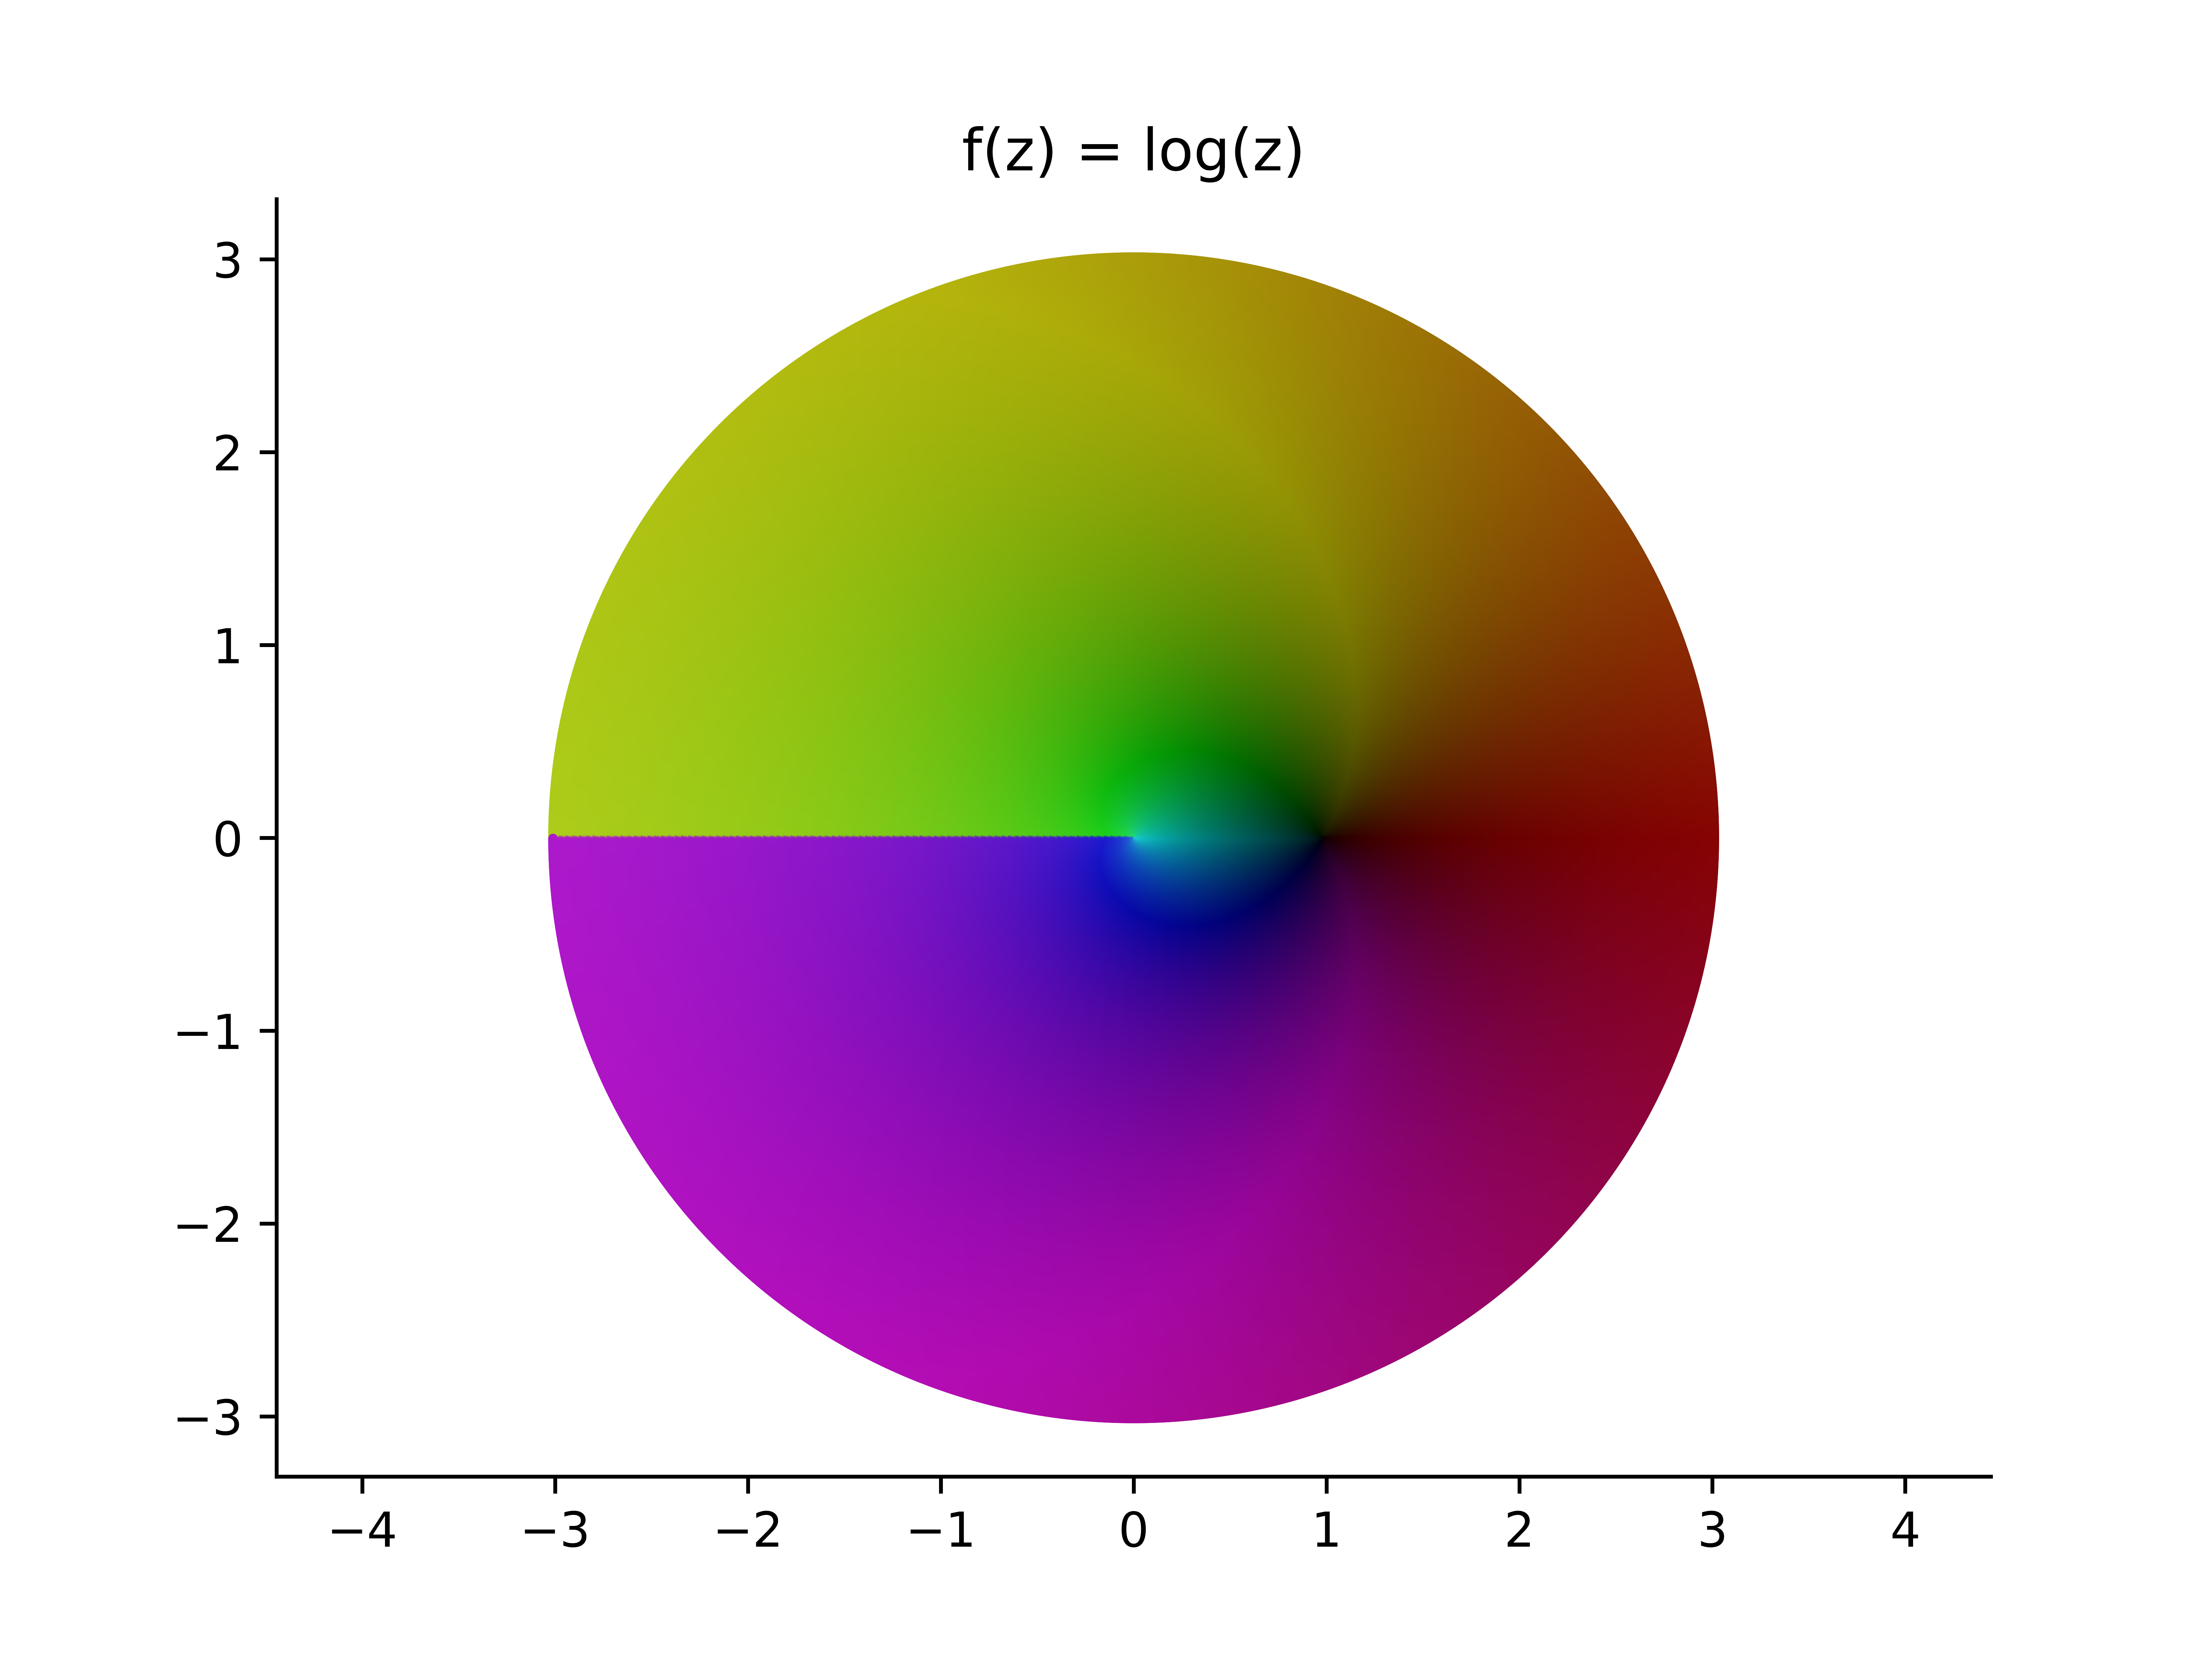
\includegraphics[width=0.7\textwidth]{../Aplicacion/log(z).png}
    \caption{Representación de la función $f(z) = \log(z)$.}
    \label{fig:log(z)}
\end{figure}

Por último, la figura \ref{fig:z^8-2z^7+2z^6-4z^5+2z^4-2z^3-5z^2+4z-4} es la representación de la función $f(z) = z^8-2z^7+2z^6-4z^5+2z^4-2z^3-5z^2+4z-4$ mediante la técnica del coloreado. Las raíces de $f$ vienen representadas por los $6$ puntos negros en el dibujo. Sin embargo, este polinomio tiene $8$ raíces de las cuales $2$ son raíces dobles. Las raíces simples ocurren en los puntos $-1$, $2$ y $\frac{(-1 \rpm i \sqrt{7})}{2}$, y las raíces dobles en $\frac{1 \rpm i \sqrt{3}}{2}$.  La región que rodea a las raíces dobles es algo más oscura que la que rodea a las raíces simples, y en las raíces dobles los colores del círculo cromático la envuelven dos veces, mientras que en las raíces simples la envuelven una sola vez. \\

Además, el dibujo también muestra que el polinomio es de grado $8$. Para $z$ de módulo grande, el término de $z^8$ domina a los otros términos, y por consiguiente la parte exterior del dibujo es similar a la representación de la función $z^8$. Esto puede observarse en que los colores del círculo cromático aparecen ocho veces. \\

\begin{figure}[!htbp]
    \centering
    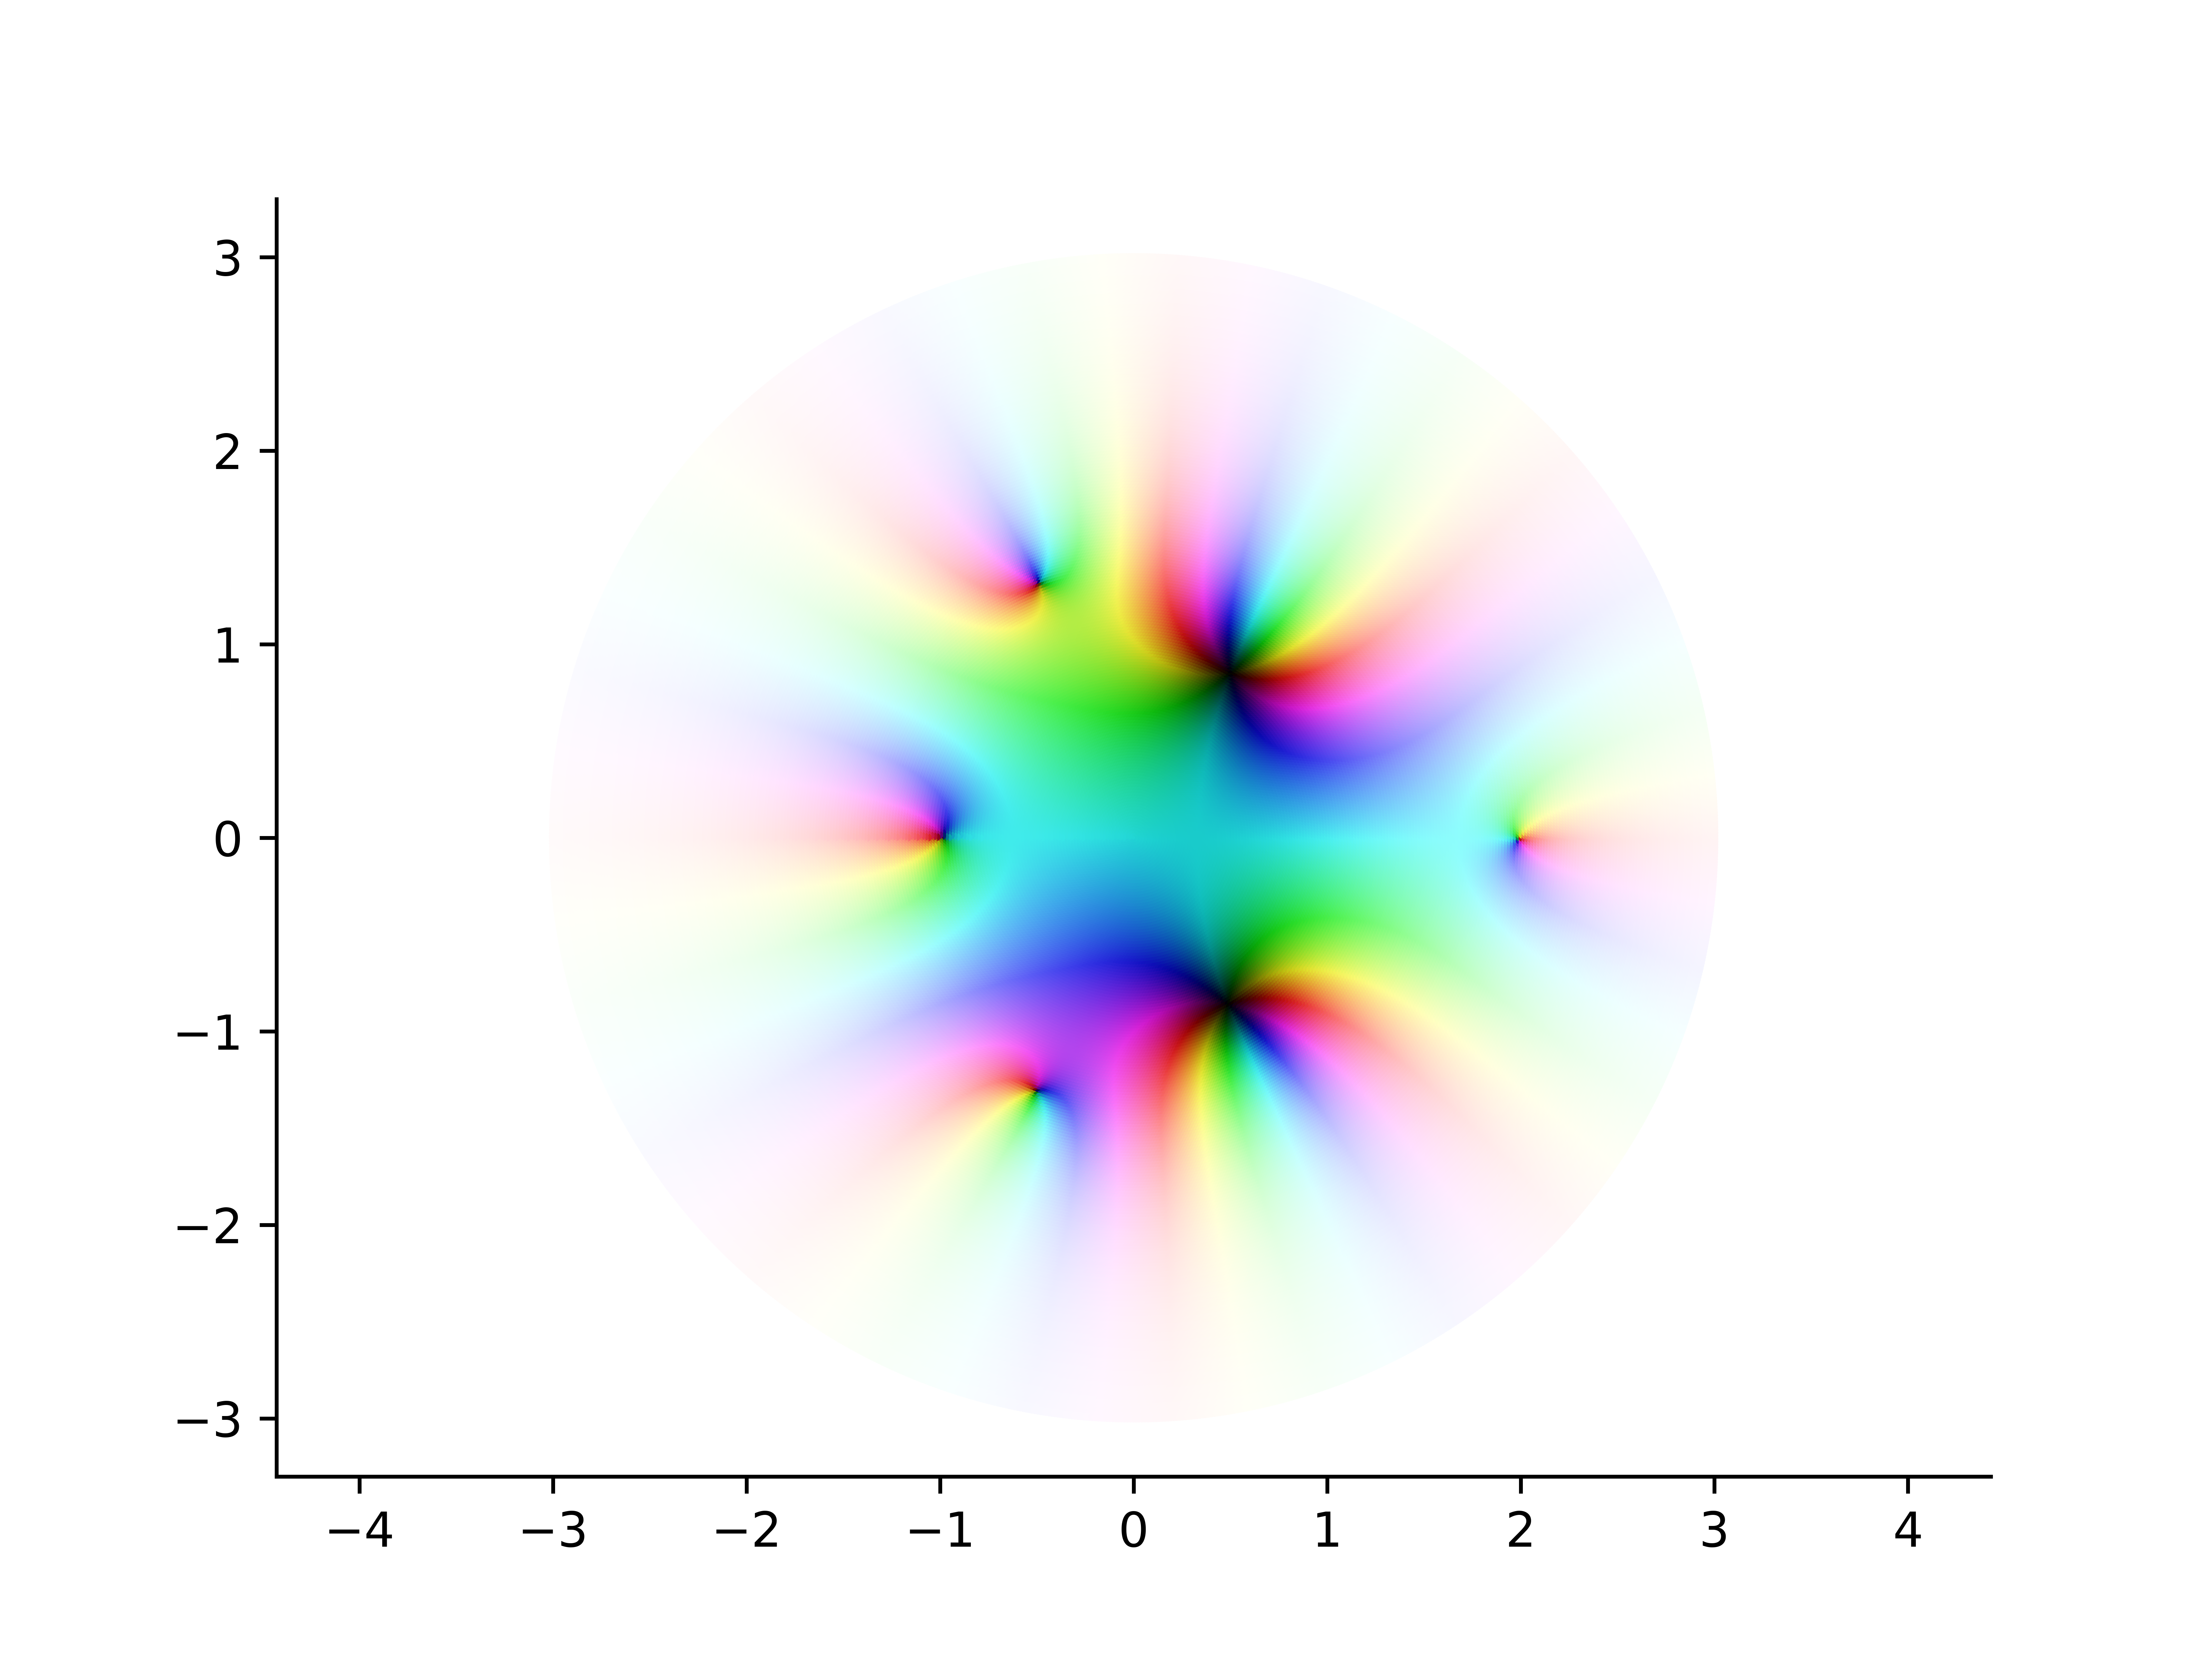
\includegraphics[width=0.7\textwidth]{../Aplicacion/z^8-2z^7+2z^6-4z^5+2z^4-2z^3-5z^2+4z-4.png}
    \caption{$f(z) = z^8-2z^7+2z^6-4z^5+2z^4-2z^3-5z^2+4z-4$}
    \label{fig:z^8-2z^7+2z^6-4z^5+2z^4-2z^3-5z^2+4z-4}
\end{figure}

Introducimos un modelo de color gracias al cual vamos a poder representar fácilmente funciones complejas siguiendo el esquema de asignación de colores explicado anteriormente. Dicho modelo se conoce como HVS (del inglés, \textit{Hue, Saturation, Value} - Tono, Saturación, Valor). \\

El primero de los atributos, que determina el tono de un color, se puede especificar por el ángulo que ocupa alrededor de un punto. Según va aumentando el ángulo, el color va variando de rojo -para los números reales positivos-, amarillo, verde, cyan, azul, magenta para volver de nuevo al rojo. Así pues el tono asociado a un número complejo está directamente relacionado con su argumento. Por otra parte, la saturación es la intensidad de un tono específico, basándose en la pureza del color: un color muy saturado es vivo e intenso, mientras que un color menos saturado es más descolorido y gris. Por último, el valor indica la cantidad de luz que tiene un color. Cuánto más oscuro sea, menor será su valor y cuánto más claro, mayor. De este modo, la saturación y el valor asociadas a un número complejo están relacionados con el módulo del mismo. \\

\begin{figure}[!htbp]
    \begin{minipage}[h]{\textwidth}
        \centering
        \parbox[c][1cm]{\textwidth}{\centering \textbf{Tono}: \\}
        \begin{tikzpicture}[x=1mm,y=1mm]
            \foreach \x in {0,0.0111,...,1}{
                \definecolor{colorhsb}{hsb}{\x, 1, 1}
                \draw[fill=colorhsb, draw=none] (\x*100,1) rectangle +(1mm,7mm);
            }
            \node[below] at (0,1){$0º$};
            \node[below] at (100,1){$360º$};
        \end{tikzpicture}
        \label{fig:hue}
        %\caption{Tono}
    \end{minipage}
    \begin{minipage}[h]{\textwidth}
        \centering
        \parbox[c][1cm]{\textwidth}{}{\centering \textbf{Saturación}: \\}
        \begin{tikzpicture}[x=1mm,y=1mm]
            \foreach \x in {0,0.0111,...,1}{
                \definecolor{colorhsb}{hsb}{1, \x, 1}
                \draw[fill=colorhsb, draw=none] (\x*100,1) rectangle +(1mm,7mm);
            }
            \node[below] at (0,1){$0º$};
            \node[below] at (100,1){$100º$};
        \end{tikzpicture}
        \label{fig:saturation}
        %\caption{Saturación}
    \end{minipage}
    \begin{minipage}[h]{\textwidth}
        \centering
        \parbox[c][1cm]{\textwidth}{\centering \textbf{Valor}: \\}
        \begin{tikzpicture}[x=1mm,y=1mm]
            \foreach \x in {0,0.0111,...,1}{
                \definecolor{colorhsb}{hsb}{1, 1, \x}
                \draw[fill=colorhsb, draw=none] (\x*100,1) rectangle +(1mm,7mm);
            }
            \node[below] at (0,1){$0º$};
            \node[below] at (100,1){$100º$};
        \end{tikzpicture}
        \label{fig:value}
        %\caption{Valor}
    \end{minipage}
    \caption{Modelo de color HSV}
    \label{fig:hsv}
\end{figure}

Los colores en Python se pueden dibujar mediante tuplas RGB de valores comprendidos entre el cero y el uno, esto es, $color \, rgb = (r, g, b)$, con $0 \leq r, g, b \leq 1$. Cada uno de estos números se corresponde con uno de los tres colores primarios: rojo (\textit{red}), verde (\textit{green}) y azul (\textit{blue}). Estos colores se representan como: $rojo = (1, 0, 0)$, $verde = (0, 1, 0)$ y $azul = (0, 0, 1)$. Además, el blanco y el negro suponen todos estos valores a cero o a uno ($blanco = (1, 1, 1)$ y $negro = (0, 0, 0)$). \\

Ahora bien, Python también admite una representación de colores por medio de tuplas HSV con valores entre el cero y el uno, es decir, $color \, hsv = (h, s, v)$, con $0 \leq h, s, v \leq 1$. Así que podremos asociar a cada número complejo una terna en el modelo de colores HSV, cuidándonos de que los valores estén dentro del rango adecuado. Además, gracias a una función de Python podemos transformar directamente un color del modelo HSV en RGB. \\

De esta manera podremos representar cualquier color en Python como combinación de su tono, saturación y brillo, que dependen a su vez del módulo y el argumento del número complejo. \\

\section{Representación de funciones. Problema de Dirichlet}

A lo largo del trabajo nos vamos a centrar en el comportamiento de funciones en el borde del disco unidad. Por ello, la representación de funciones se realiza en discos centrados en $0$ de radio arbitrario, siendo $1$ el valor por defecto. La propia forma del dominio sugiere tomar un mallado circular y evaluar la función en cada punto. \\

La aplicación que se ha desarrollado tiene tres funcionalidades diferentes. En primer lugar, permite representar funciones complejas en un disco de radio determinado, como ya se ha mostrado en las figuras de la sección anterior, cuyas representaciones han sido obtenidos al ejecutar el programa realizado. \\

Por otra parte, también se puede resolver el problema de Dirichlet para el disco haciendo uso de la integral de Poisson. Dada una función $f$ definida en el borde del disco, la solución dada por la integral de Poisson definirá una función armónica en el disco abierto. Además, si $f$ es una función continua, la solución será también una función continua en el disco cerrado, que coincidirá con $f$ en el borde del disco. \\

La función $f$ que recibe el programa parametriza el borde del disco en función del argumento. Así pues, para poder definir funciones con mayor facilidad, su dominio de definición es $[-\pi, \pi]$ de manera que $\theta \in [-\pi, \pi]$ se corresponde con el punto $z = e^{i \theta} = \cos(\theta) + i \sen(\theta) \in \partial \disk$. \\

Podemos utilizar la representación de funciones que se ha desarrollado para comprobar que la integral de Poisson se comporta como se espera cuando la parametrización dada se corresponde, en el borde, con la función que se va a dibujar. A continuación se pueden observar algunos ejemplos. \\

La figura \ref{fig:comp_e^z} se corresponde con la extensión al disco de la función $f : [-\pi, \pi] \to \complex, t \to e^{10 \cos(t)+10i \sen(t)}$. A su vez, esta función parametriza el borde del disco de tal manera que cada punto $t \in [-\pi, \pi]$ se corresponde con un punto $z = e^{i \theta} = \cos(\theta) + i \sen(\theta) \in \partial \disk$. Deshaciendo este cambio, obtenemos que la función $f$ se puede escribir como $f: \partial \disk \to \complex, z \mapsto e^{10z}$. Volviendo a la figura \ref{fig:e^z} podemos comprobar que se trata de la misma representación. \\

\begin{figure}[!htbp]
    \centering
    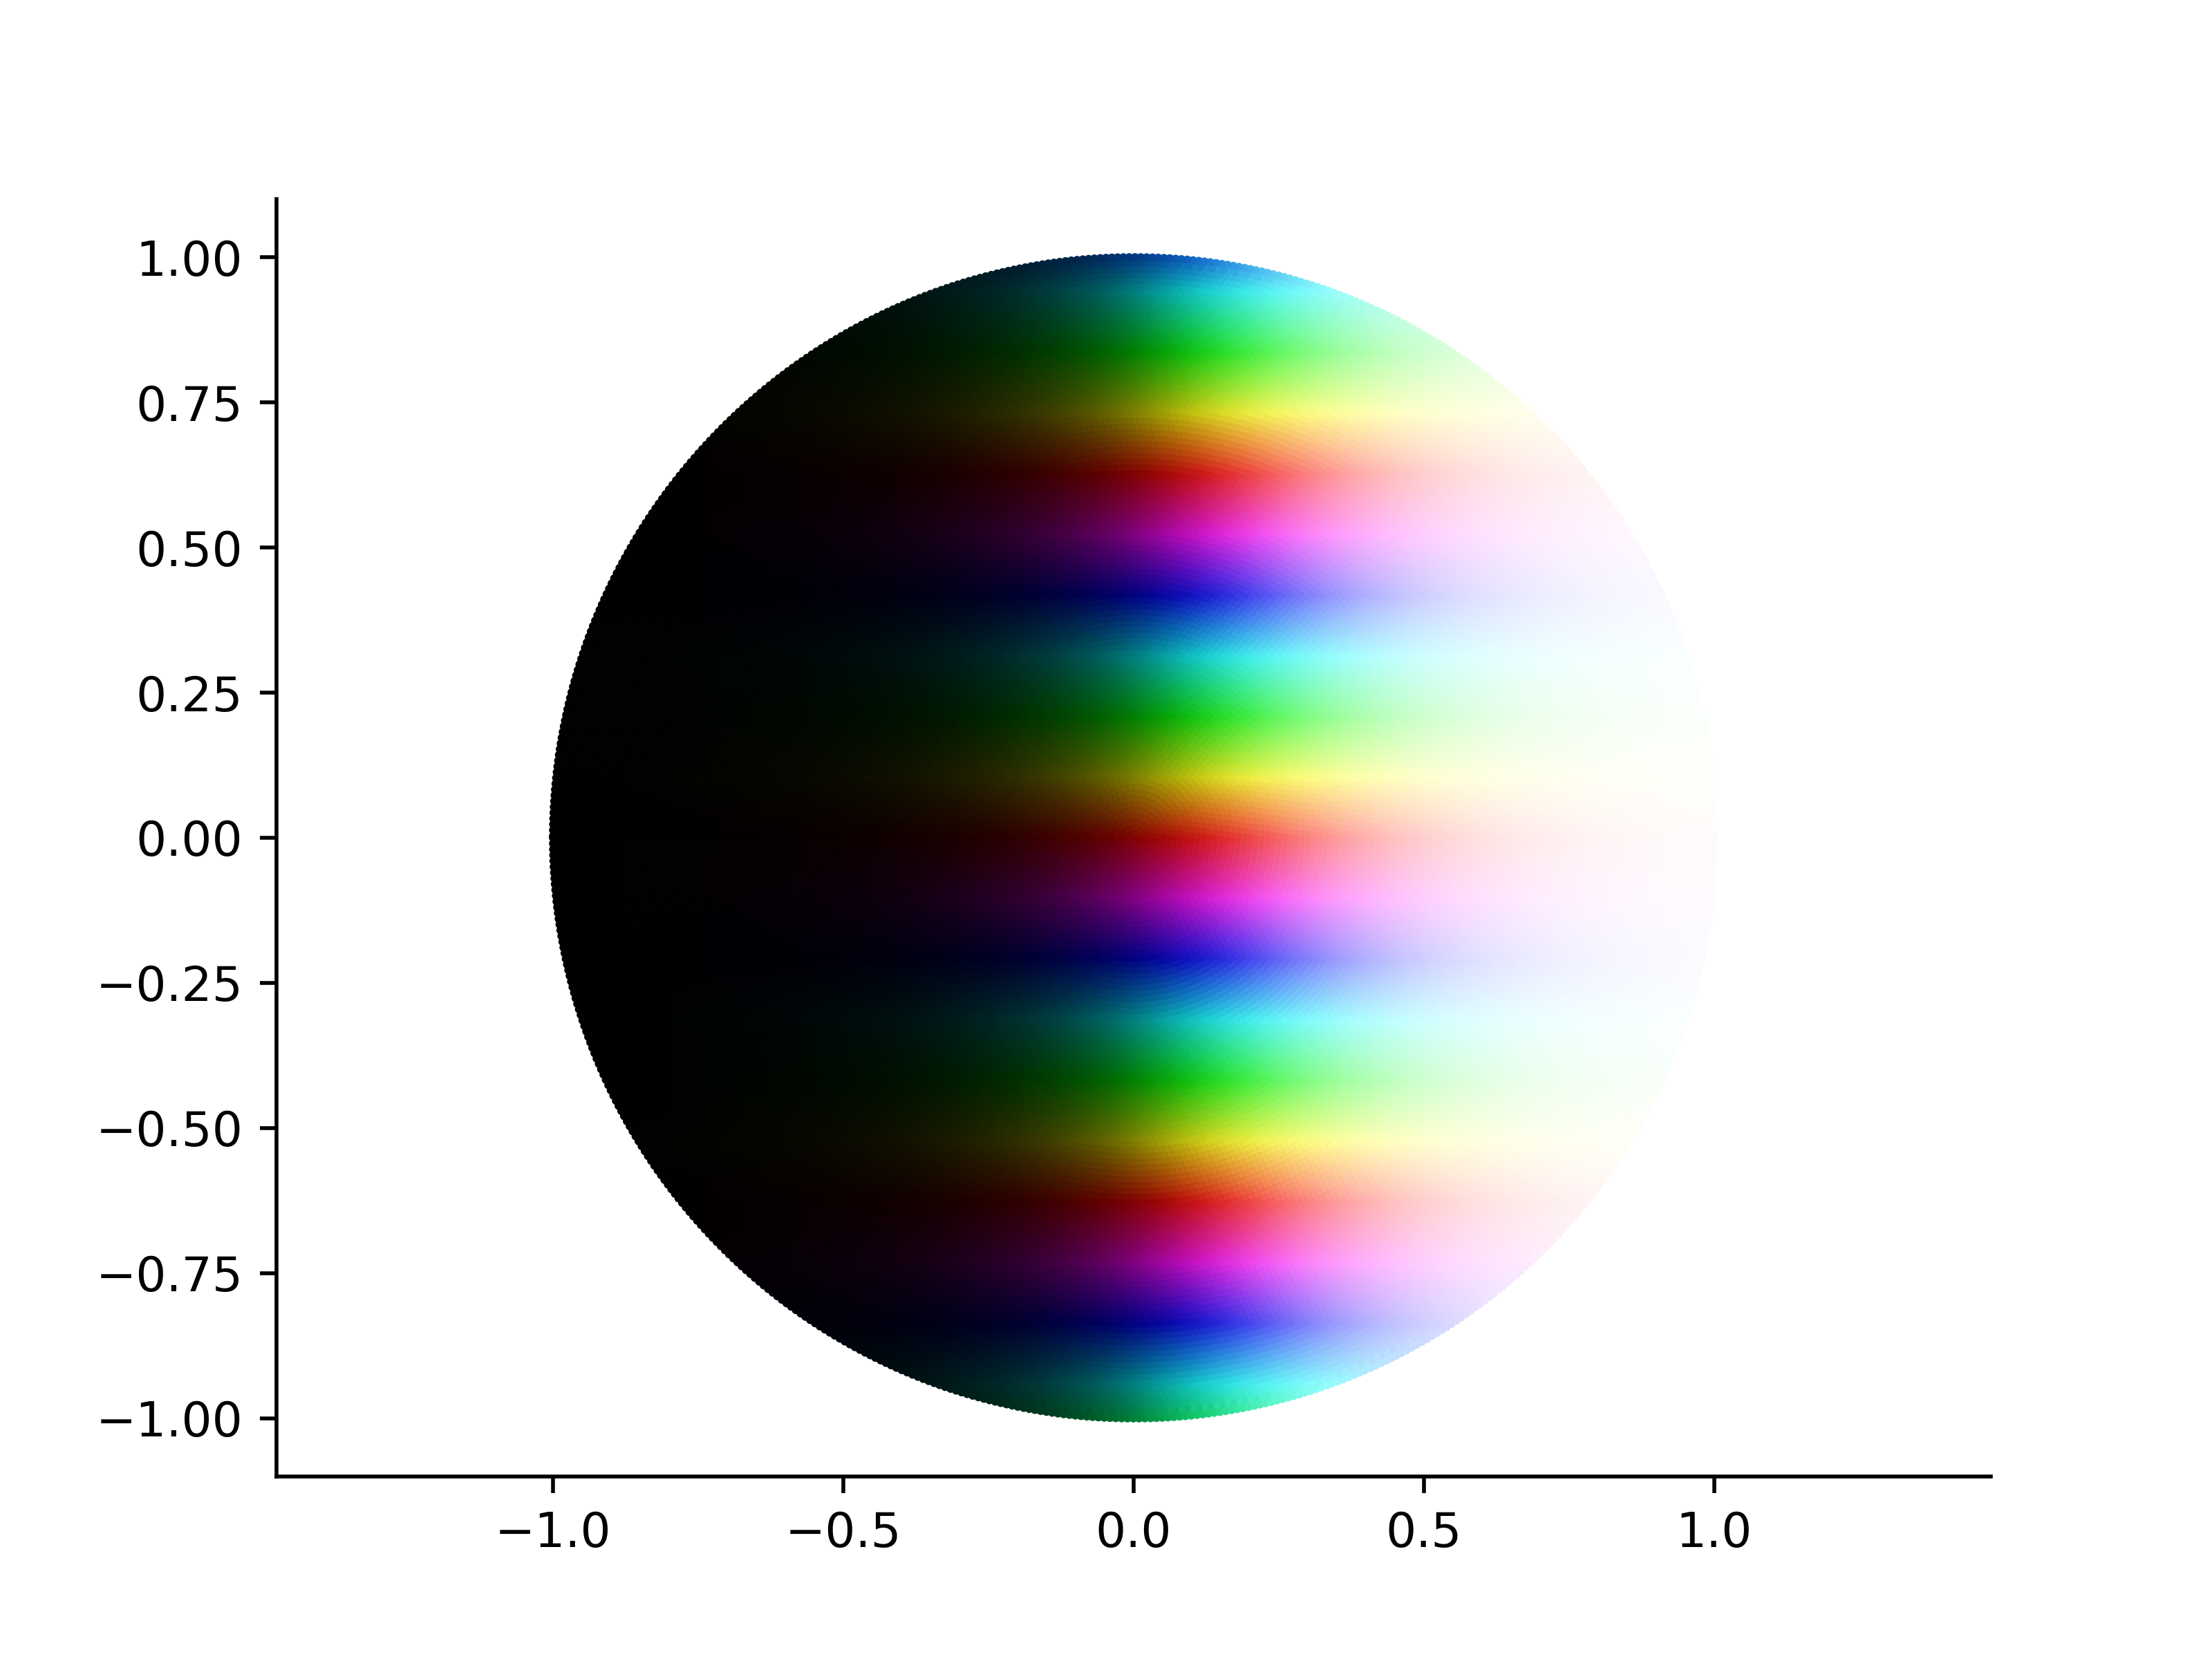
\includegraphics[width=0.7\textwidth]{../Aplicacion/e^(10cos(t)+10isen(t)).png}
    \caption{Extensión al disco de la función $f(t) = e^{10 \cos(t)+10i \sen(t)}$.}
    \label{fig:comp_e^z}
\end{figure}

La figura \ref{fig:comp_z} representa la extensión al disco de la función $f: [-\pi, \pi] \to \complex, t \to 10(\cos(t)+10i \sen(t))$. Deshaciendo este cambio como en el ejemplo anterior, tenemos que la función $f$ se puede escribir de la siguiente manera $f: \partial \disk \to \complex, z \mapsto 10z$. De nuevo, si nos fijamos en la figura \ref{fig:z} podemos observar que coinciden. \\

\begin{figure}[!htbp]
    \centering
    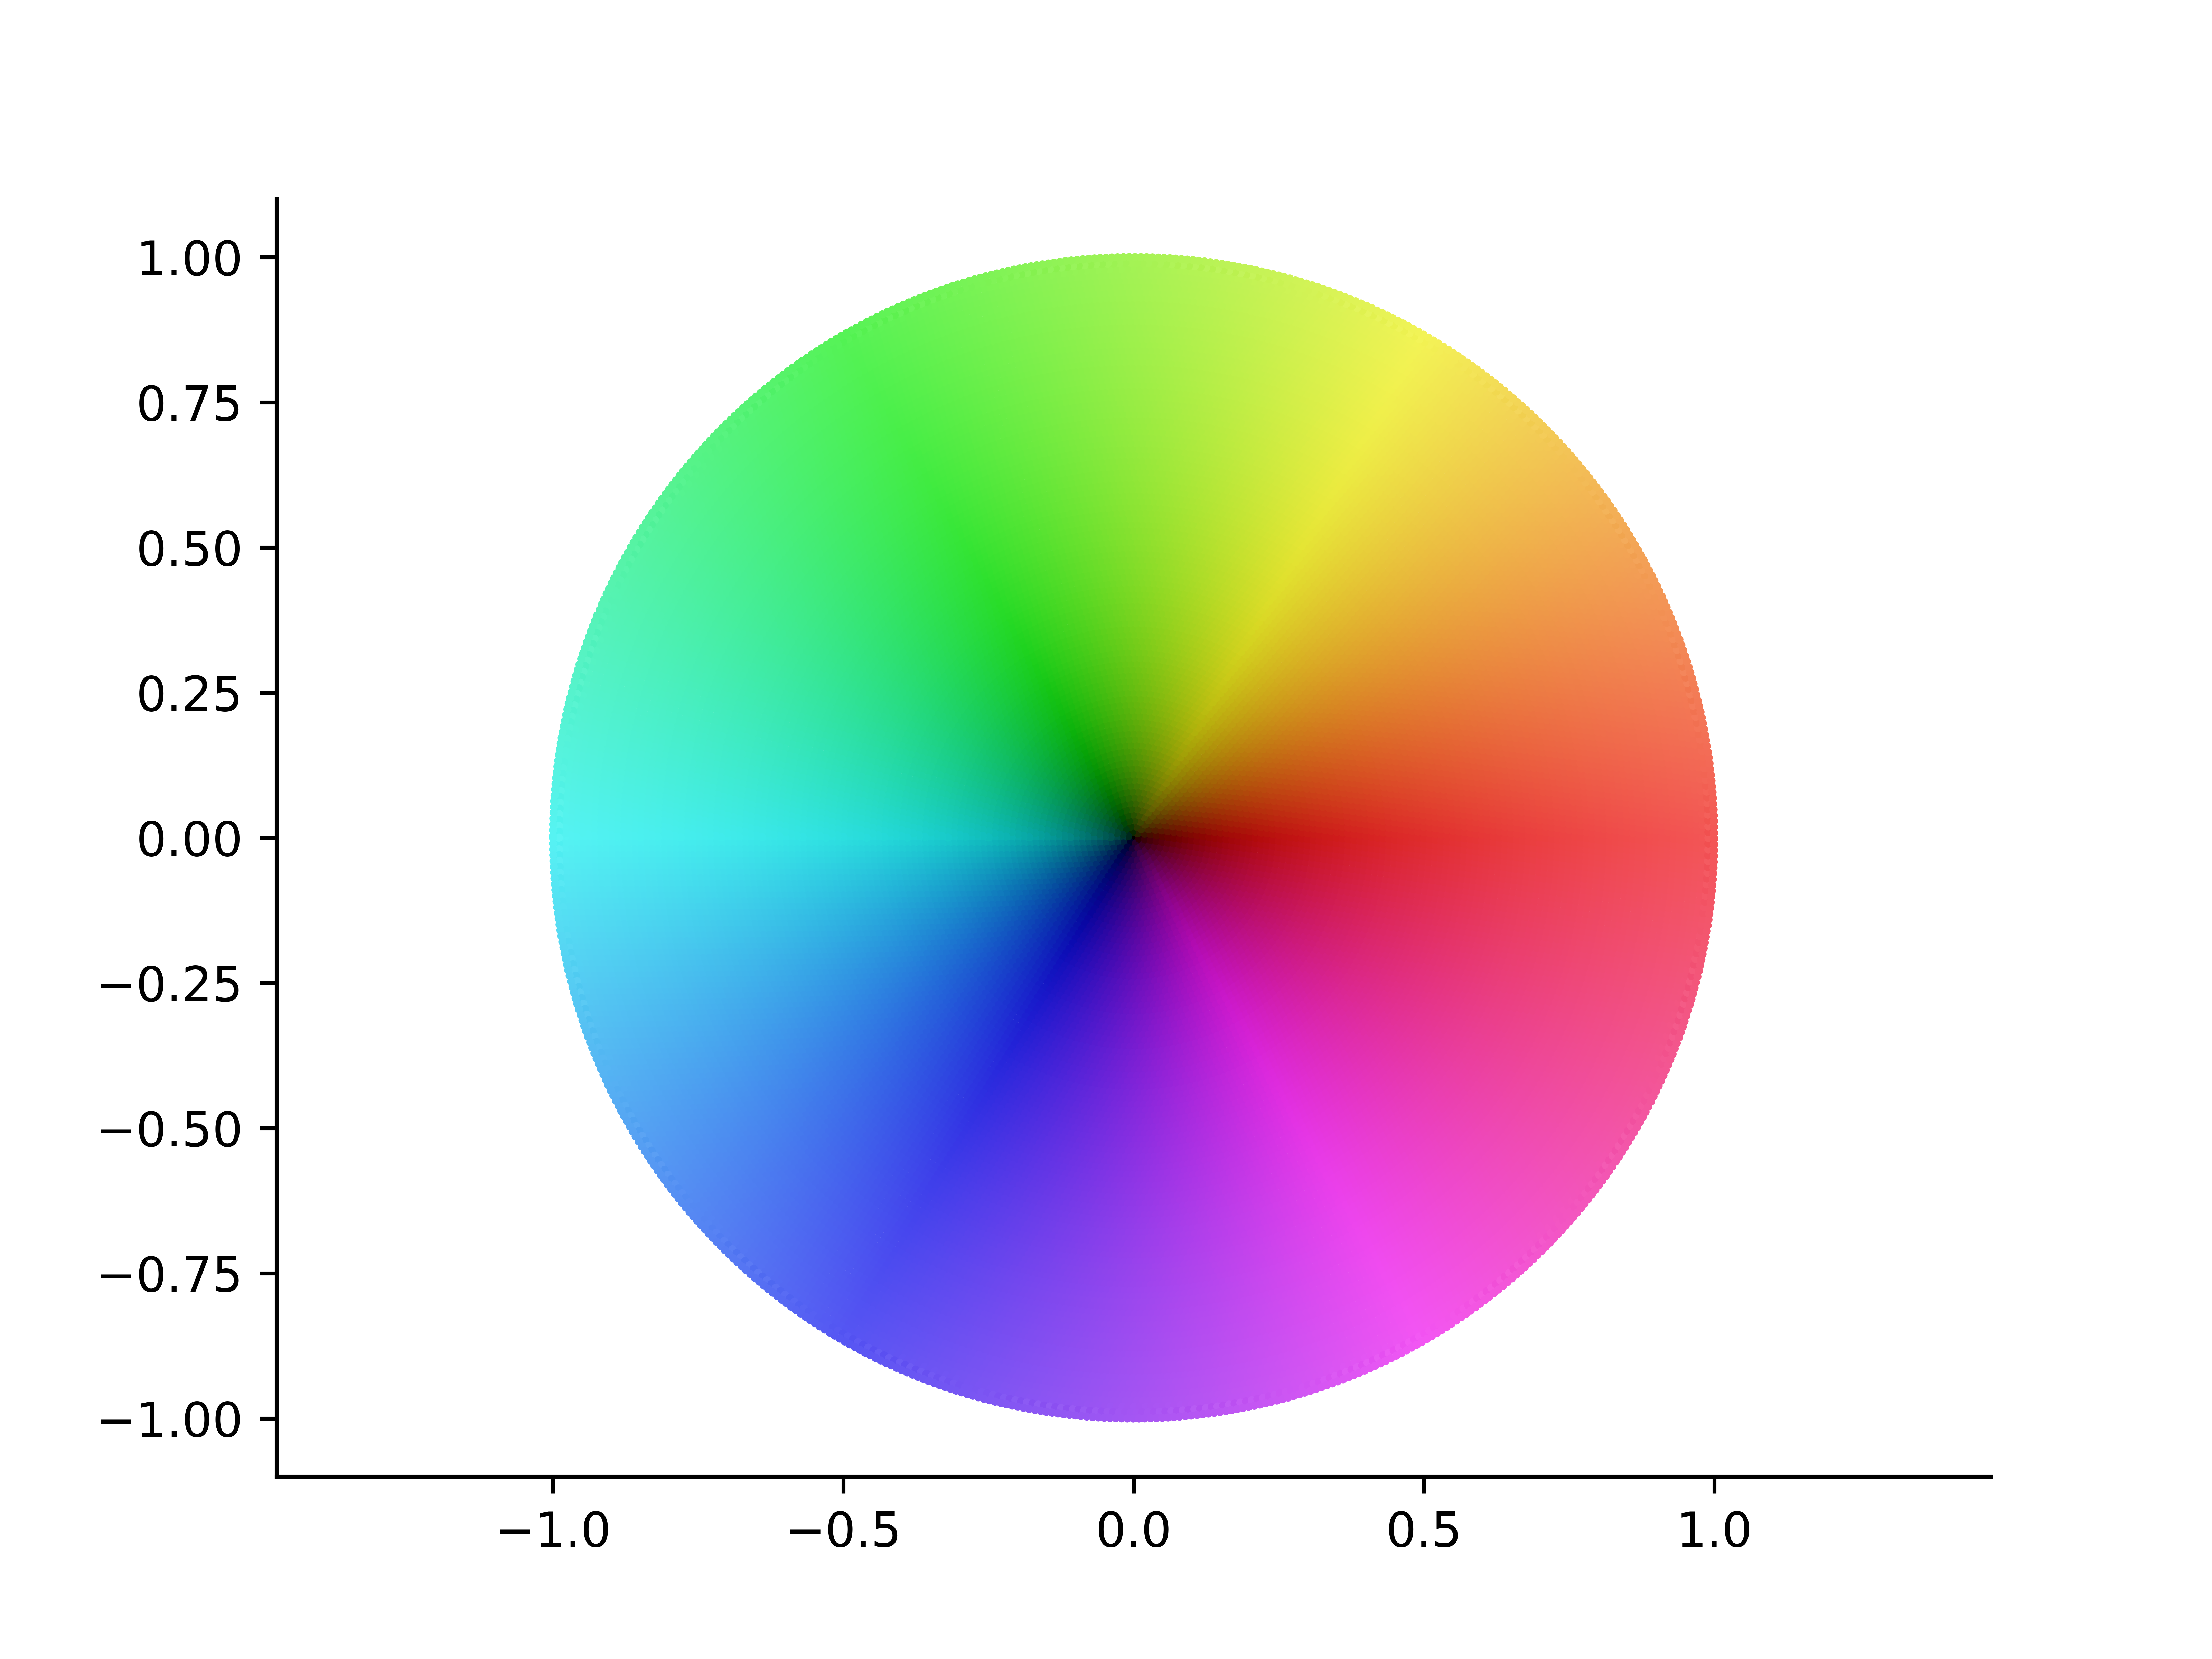
\includegraphics[width=0.7\textwidth]{../Aplicacion/10cos(t)+10isen(t).png}
    \caption{Extensión al disco de la función $f(t) = 10(\cos(t) + i \sen(t))$.}
    \label{fig:comp_z}
\end{figure}

La figura \ref{fig:comp_z^3} muestra la extensión al disco de la función $f: [-\pi, \pi] \to \complex, t \to (5\cos(t)+5i \sen(t))^3$ que se corresponde con  $f: \partial \disk \to \complex, z \mapsto (5z)^3$. Esta representación coincide con la que se observa en la figura \ref{fig:z^3}. \\

\begin{figure}[!htbp]
    \centering
    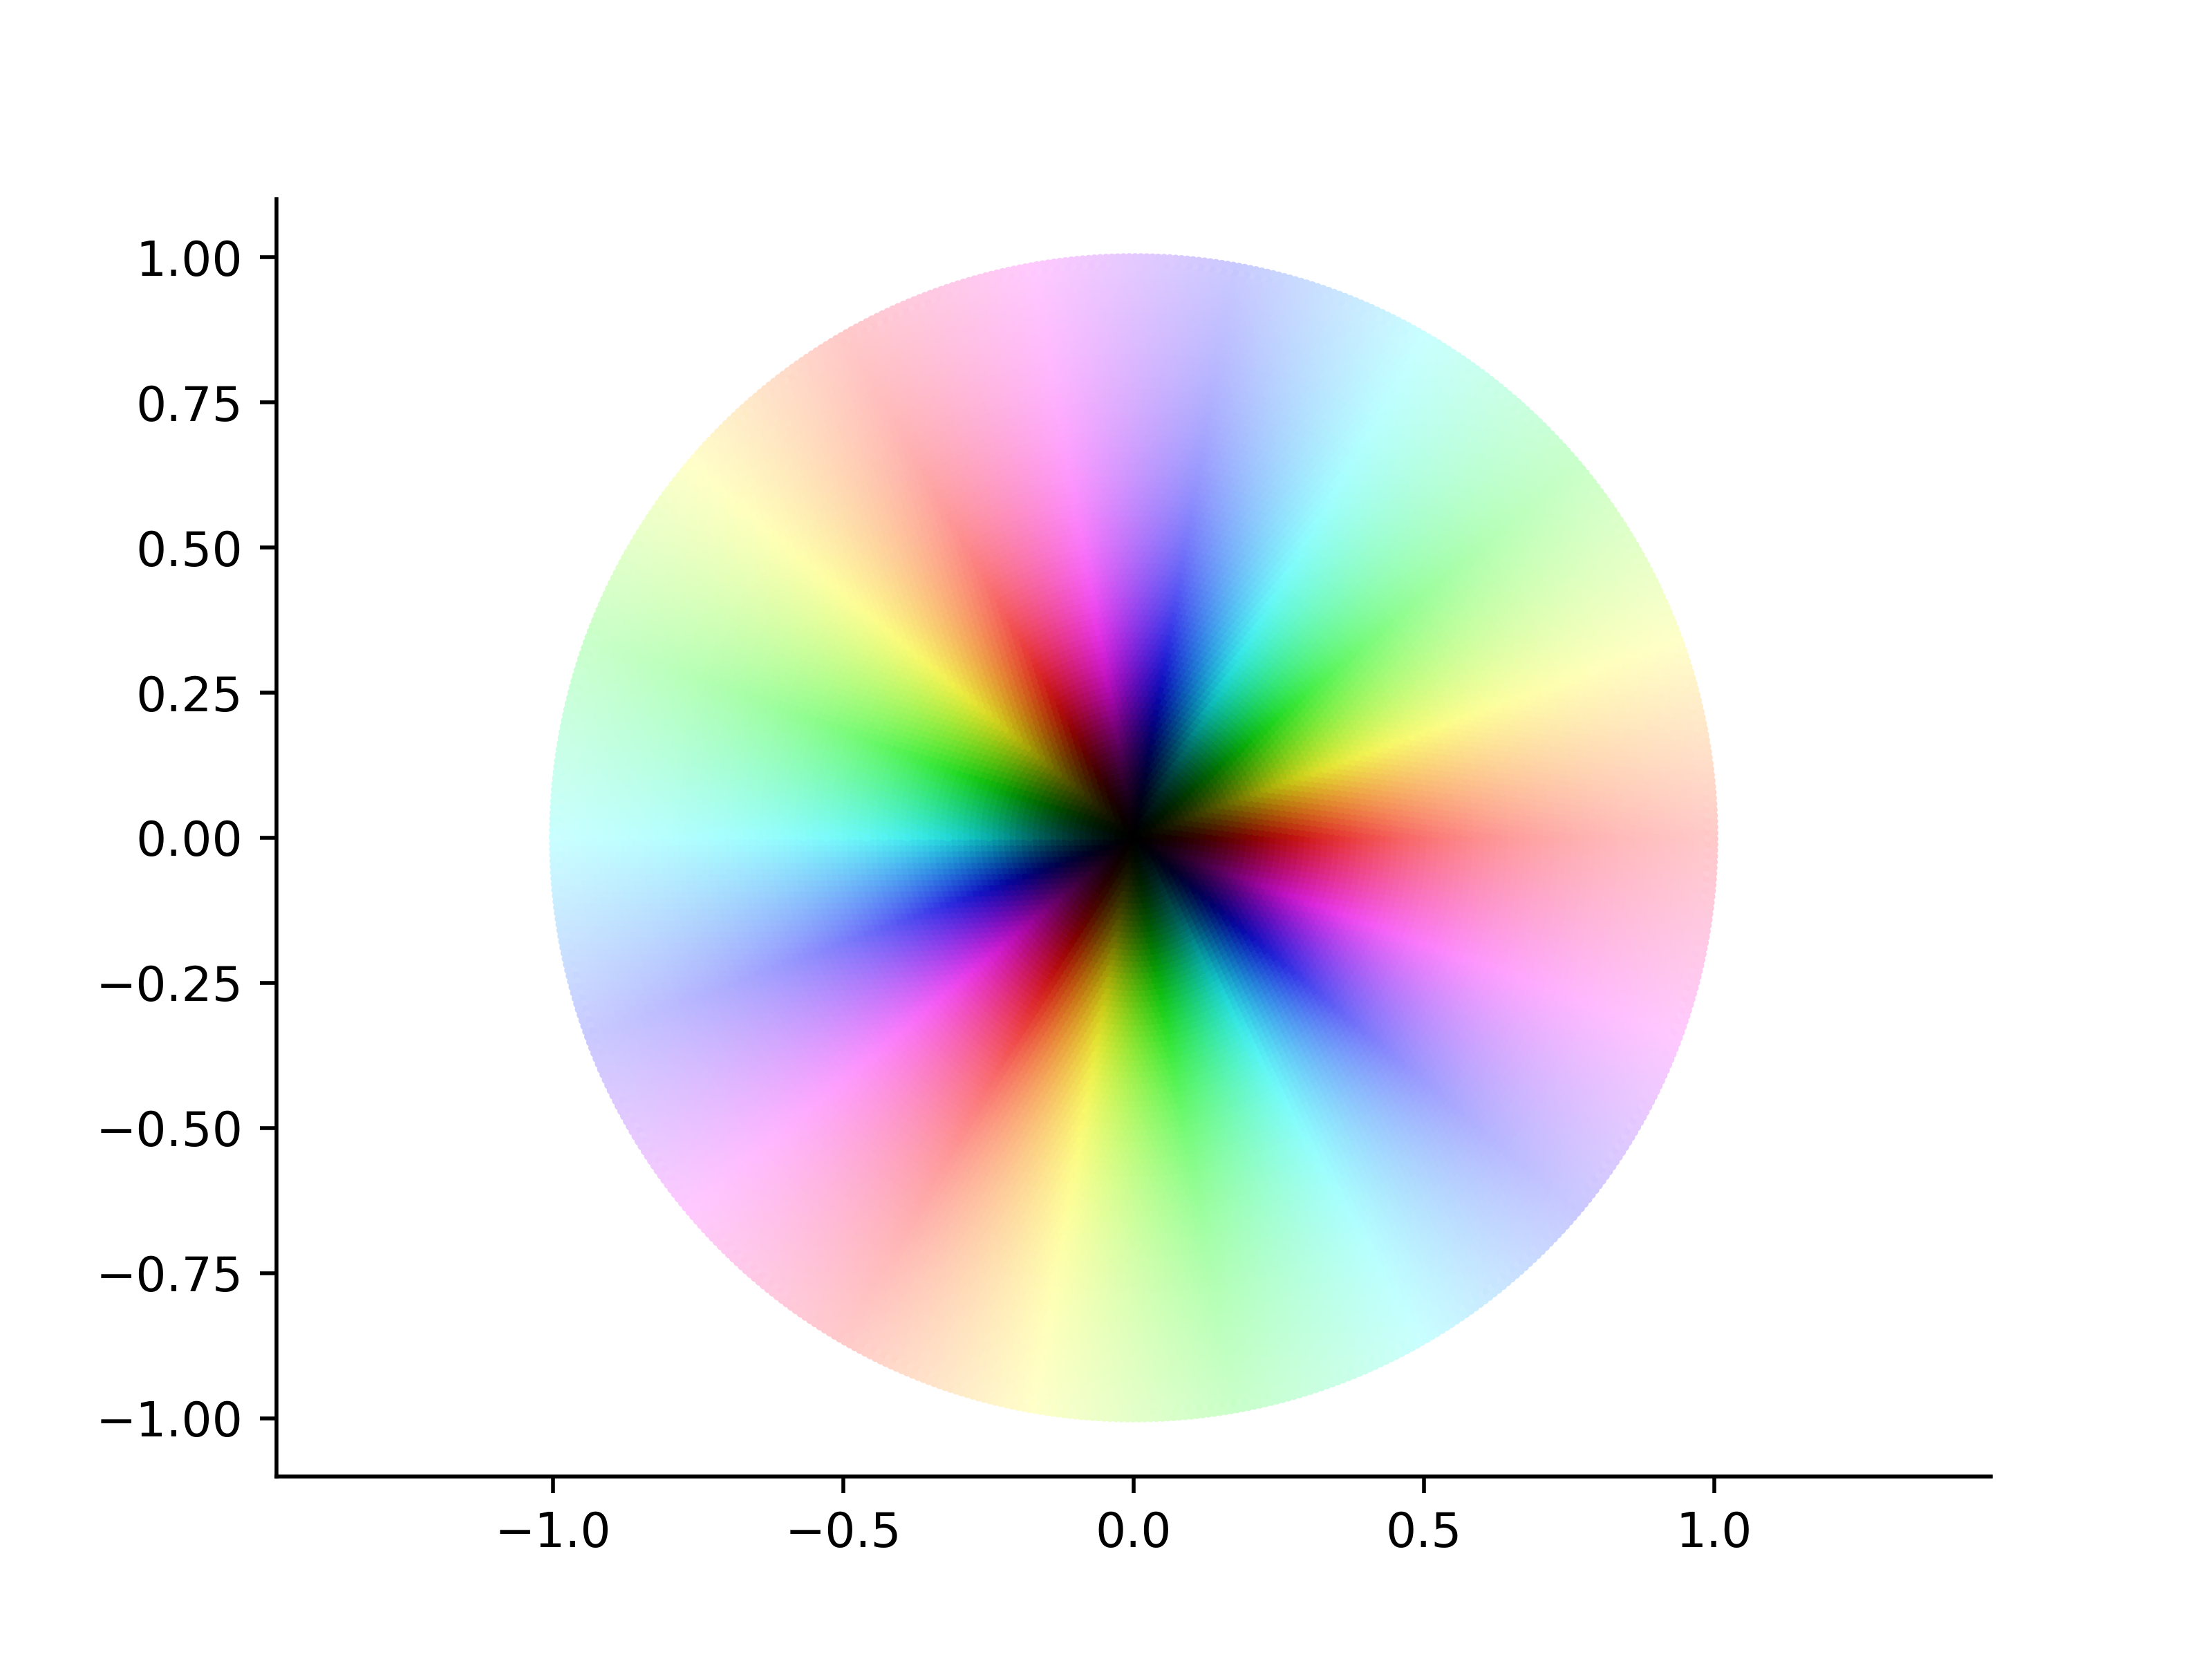
\includegraphics[width=0.7\textwidth]{../Aplicacion/(5cos(t)+5isen(t))^3.png}
    \caption{Extensión al disco de la función $f(t) = (5\cos(t)+ 5i \sen(t))^3$.}
    \label{fig:comp_z^3}
\end{figure}

Por último, la figura \ref{fig:comparacion4} se corresponde con la extensión al disco de la función $f: [-\pi, \pi] \to \complex, t \to \cos^2(t)-\sen^2(t)$ que también puede escribirse como $f: \partial \disk \to \complex, z \mapsto \Re(z^2)$. \\

\begin{figure}[!htbp]
    \centering
    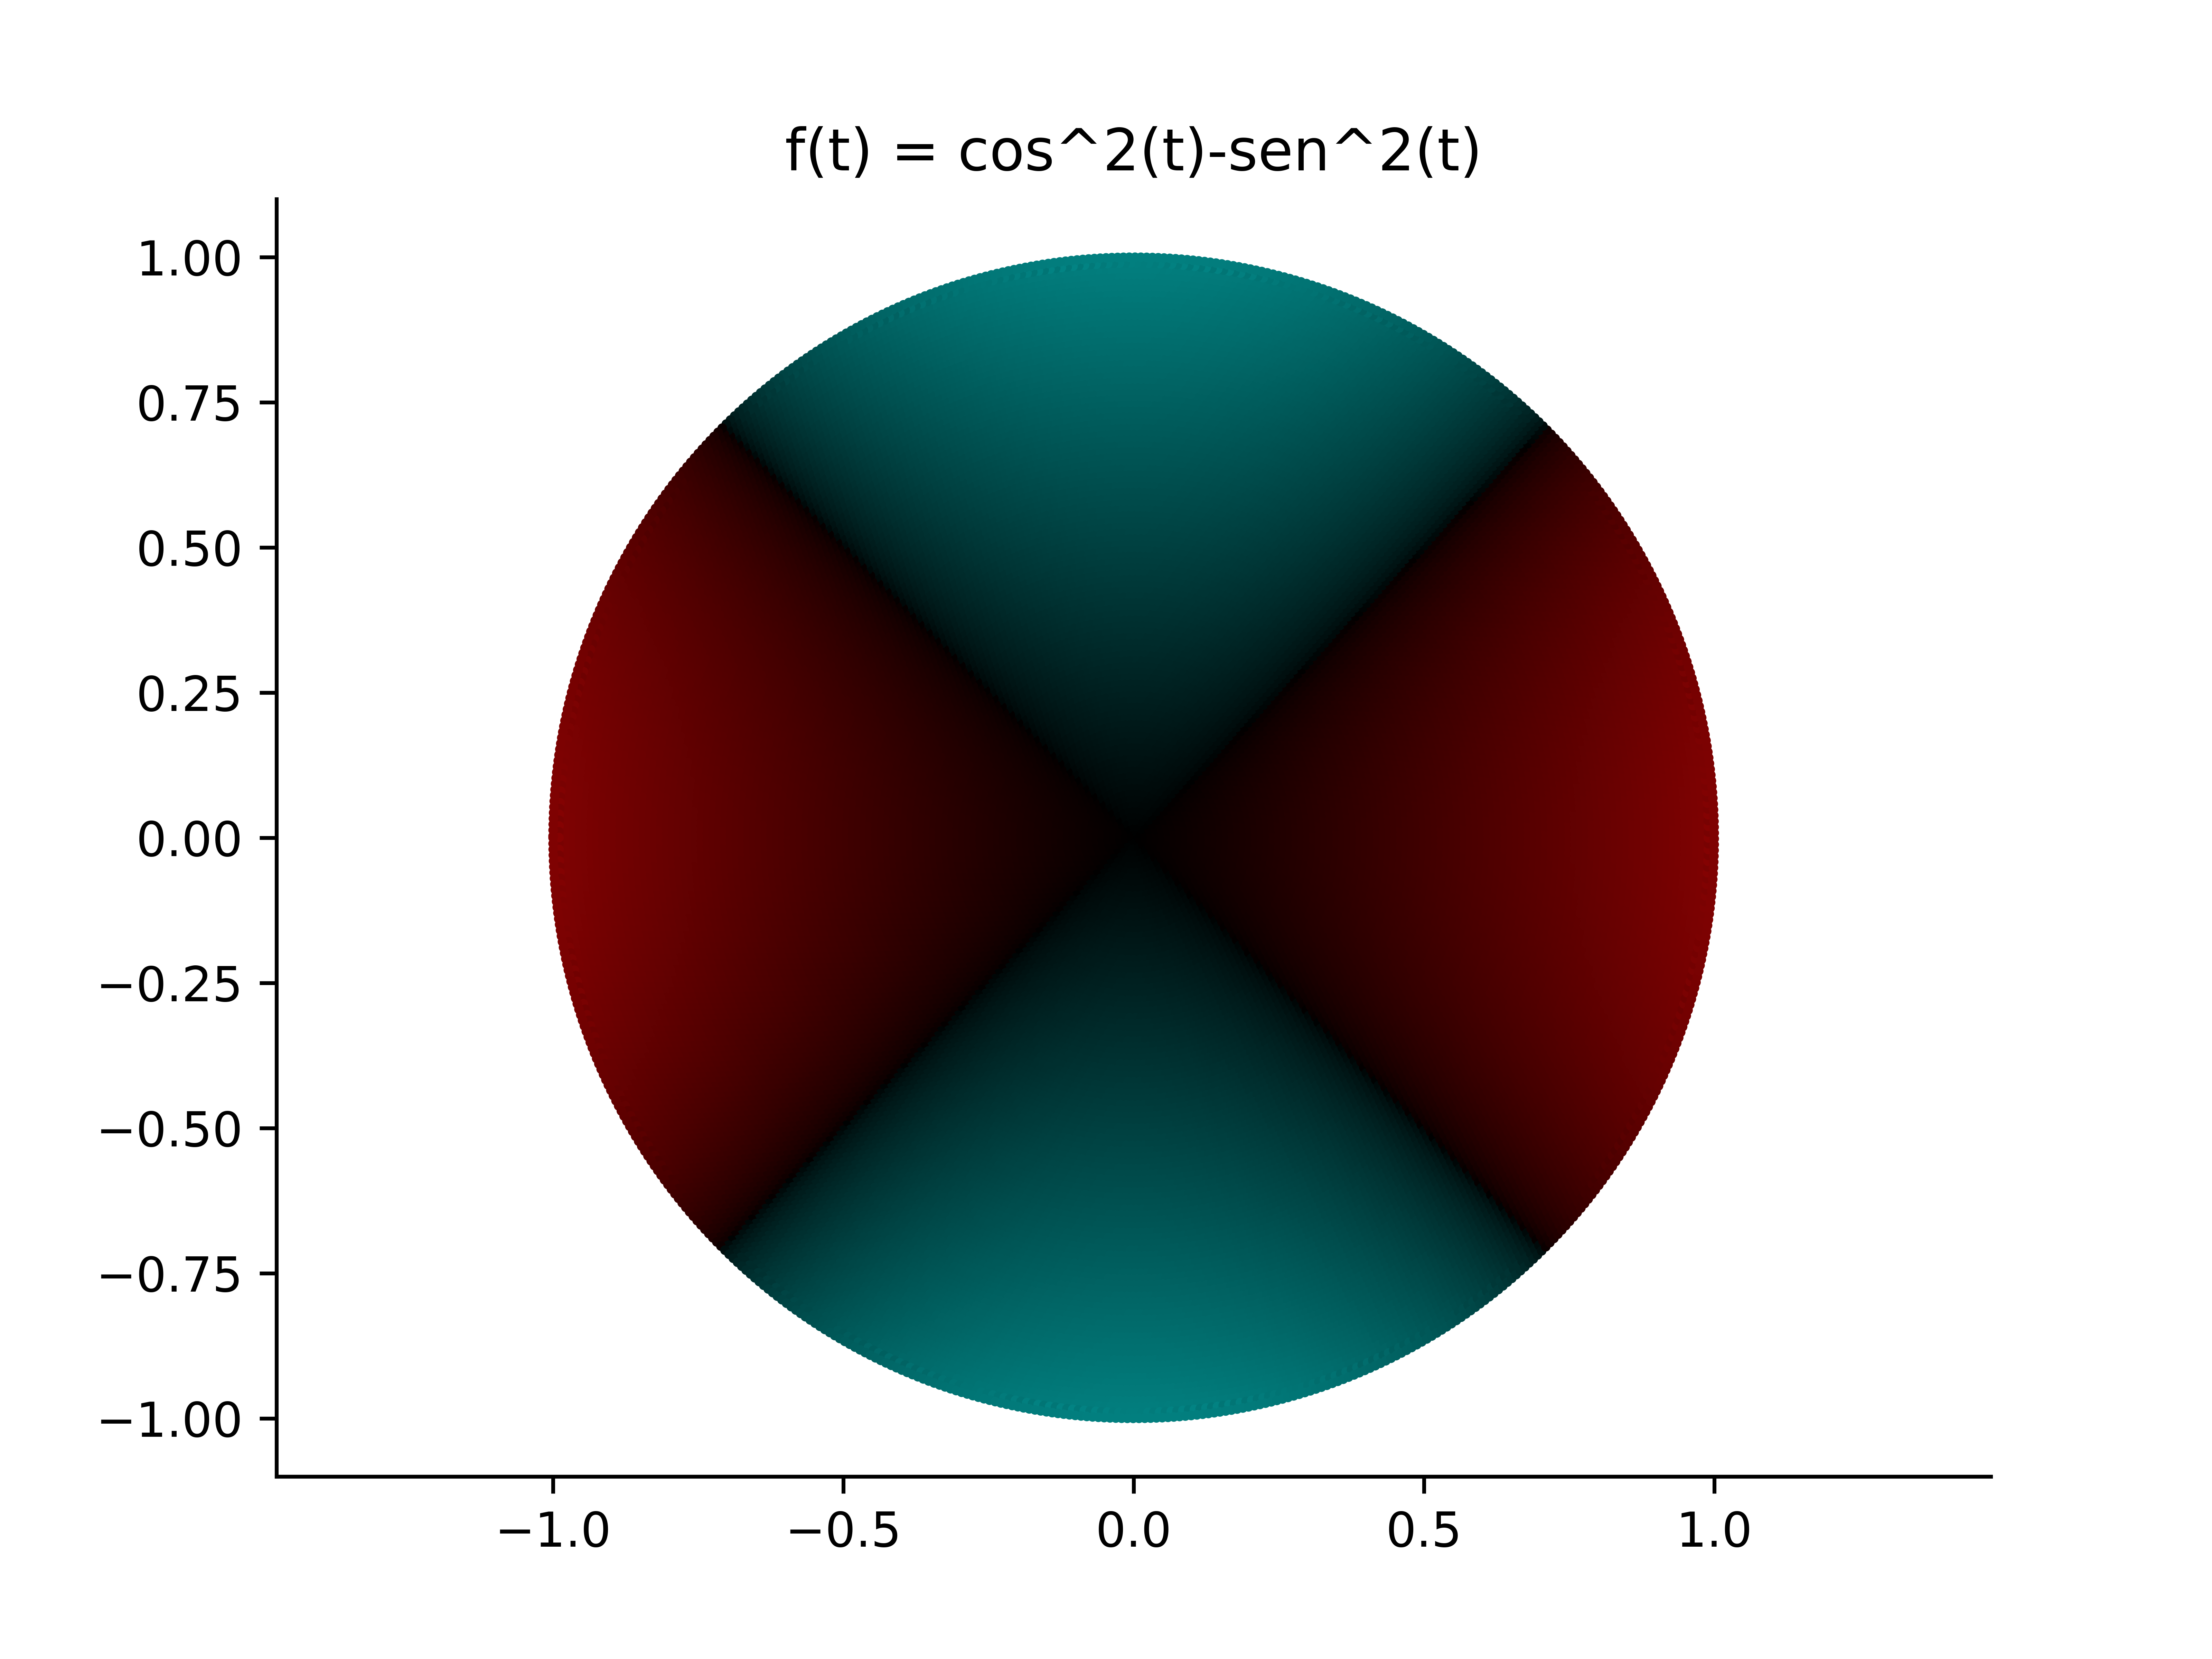
\includegraphics[width=0.7\textwidth]{../Aplicacion/cos^2(t)-sen^2(t).png}
    \caption{Extensión al disco de la función $f(t) = \cos^2(t) - \sen^2(t)$.}
    \label{fig:comparacion4}
\end{figure}

Esta misma comprobación se puede llevar a cabo mediante la última funcionalidad de la aplicación que permite representar la diferencia de funciones. Por lo tanto, si el cálculo de la integral de Poisson fuera perfecto, el dibujo resultante sería negro en su totalidad. Esto se consigue en la mayoría de los ejemplos, con funciones acotadas por valores no muy grandes. \\

Sin embargo, debido a errores numéricos, este cálculo no es totalmente exacto y presenta algunas inexactitudes sobre todo en puntos cercanos al borde del disco o cuyo módulo, a través de la función, es grande. Podemos ver esto reflejado en la figura \ref{fig:diferencia} que muestra la diferencia entre las figuras \ref{fig:comp_e^z} y \ref{fig:e^z}. \\

\begin{figure}[!htbp]
    \centering
    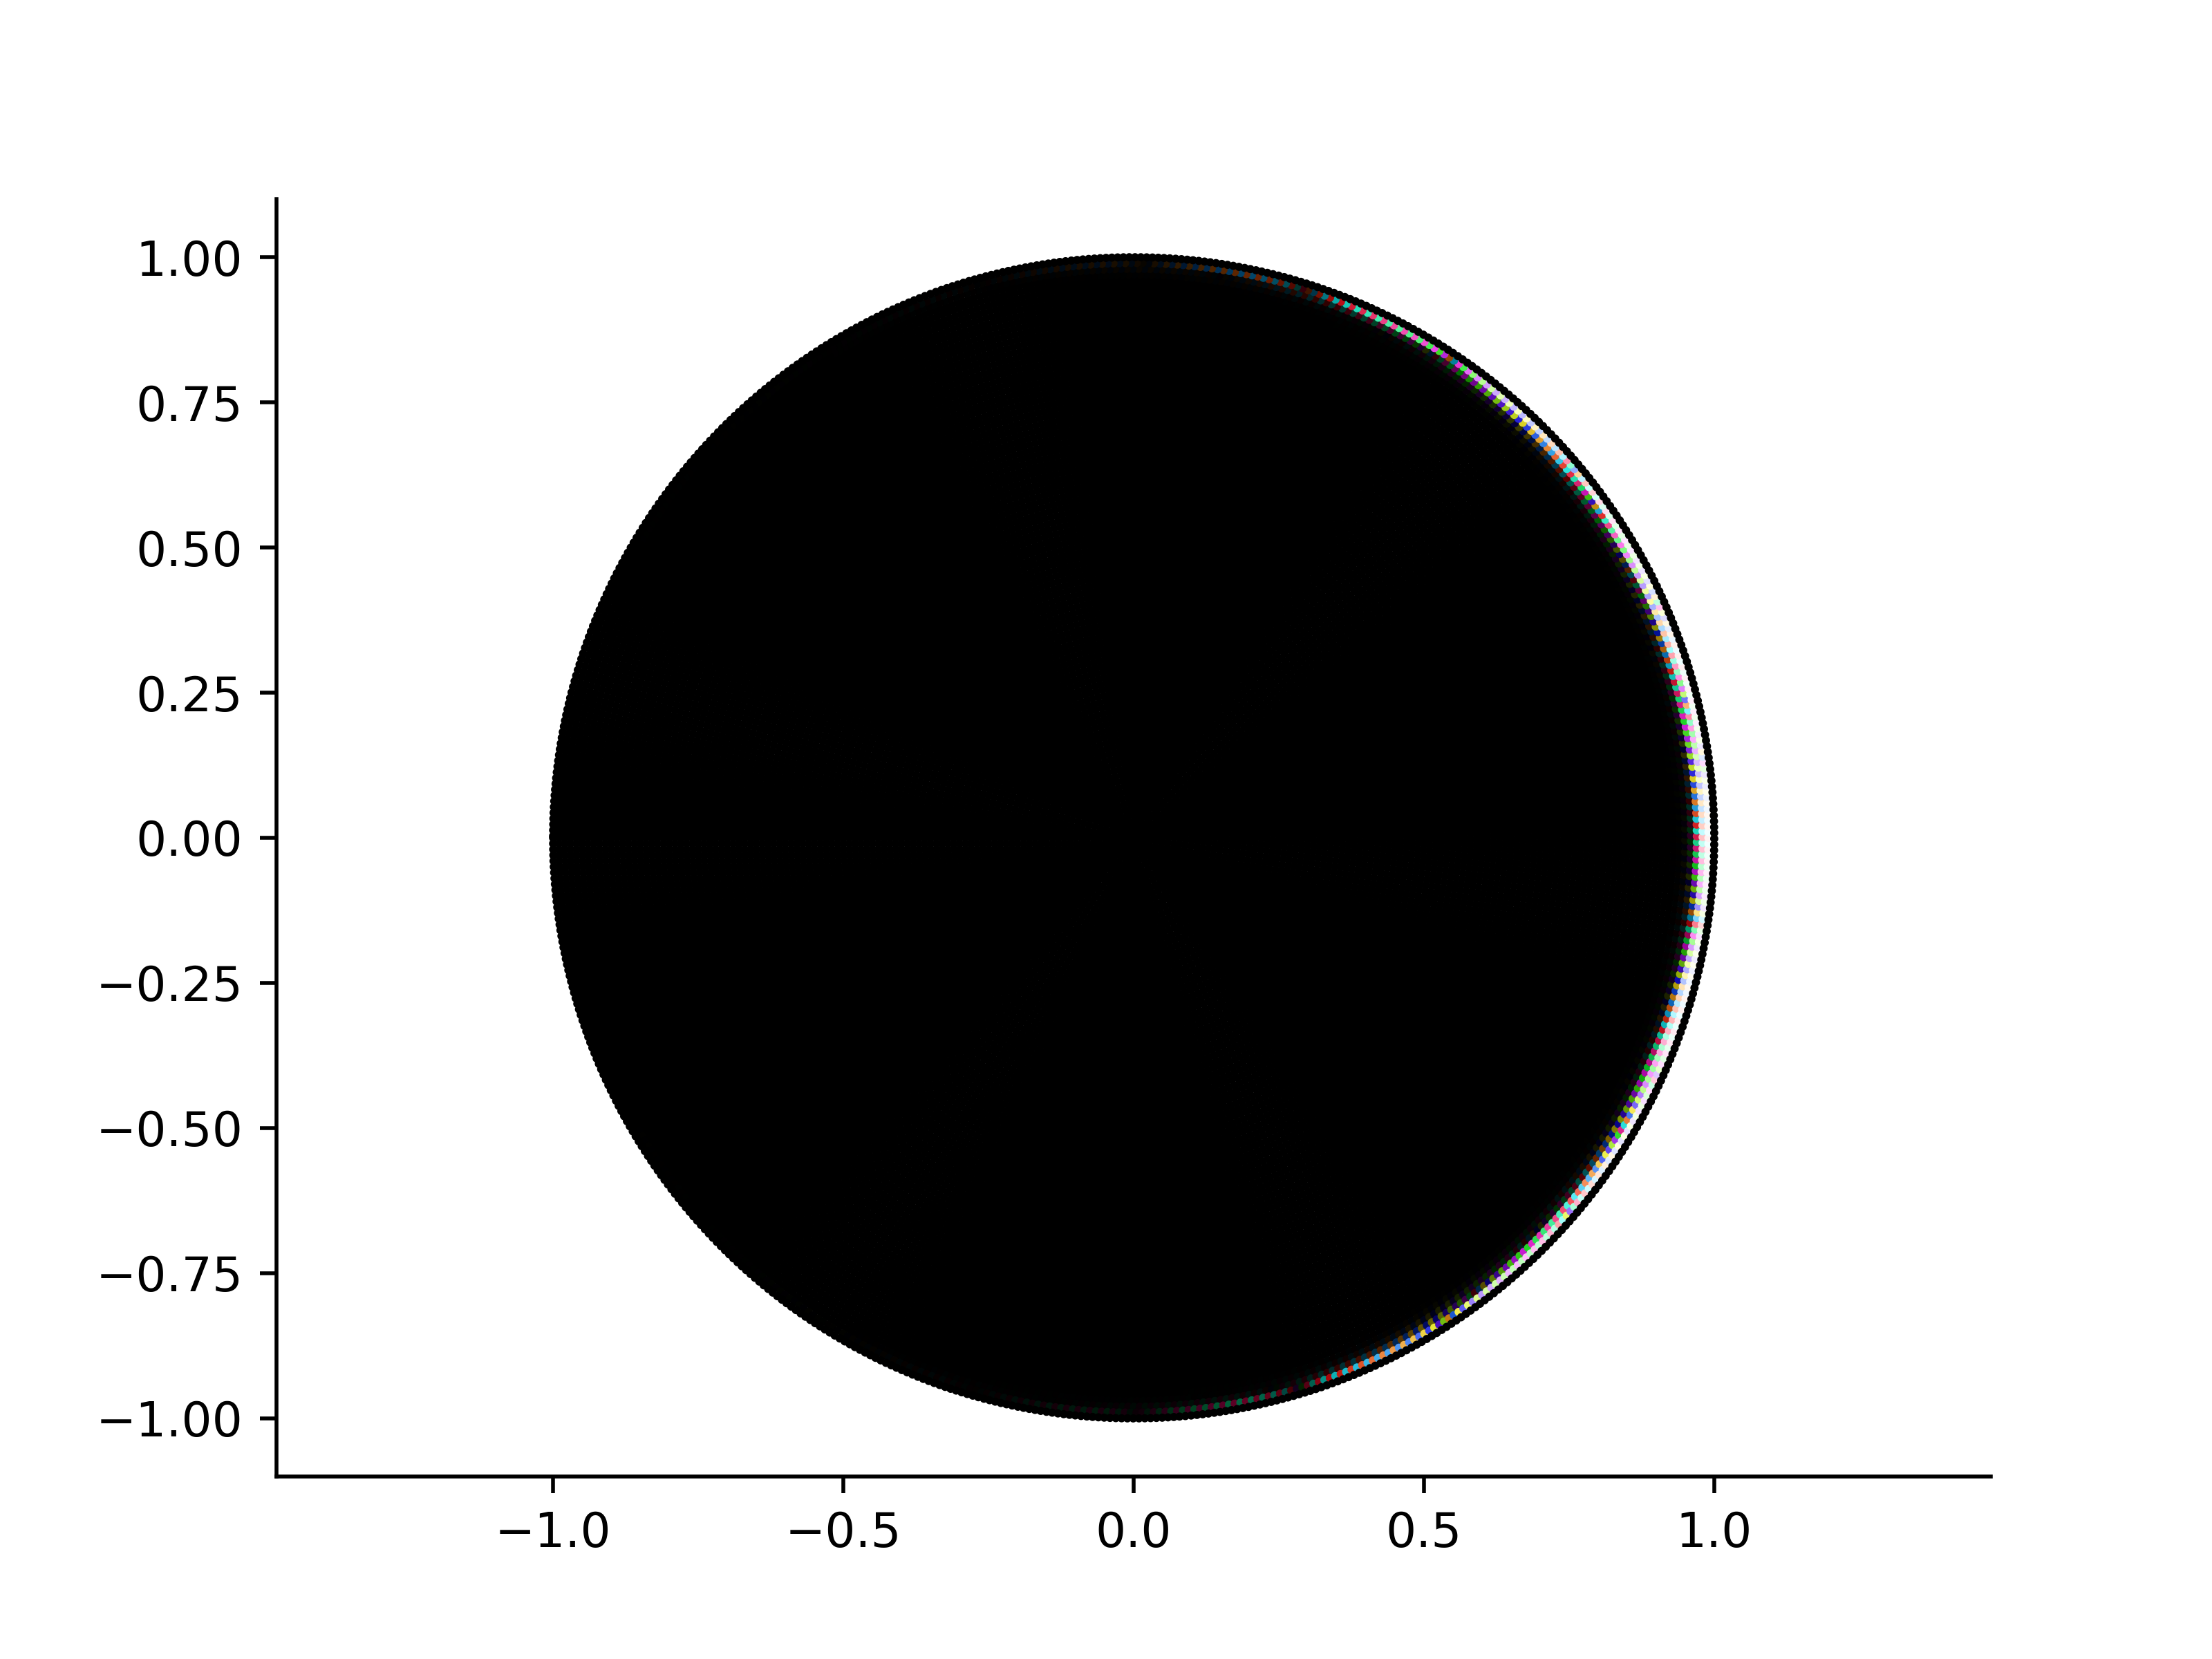
\includegraphics[width=0.7\textwidth]{../Aplicacion/diff_e^z.png}
    \caption{Diferencia entre las figuras \ref{fig:comp_e^z} y \ref{fig:e^z}.}
    \label{fig:diferencia}
\end{figure}

Como hemos comentado previamente, $f$ ha de ser continua para que se pueda extender con continuidad al disco cerrado. Pero, ¿qué pasa cuando no lo es? El resultado será una función con parte real e imaginaria armónicas en el interior (no necesariamente una conjugada de la otra) pero que no se puede prolongar con continuidad a la frontera, como es lógico. Además, si $f$ es continua a trozos, la función que se obtiene a partir de ella es armónica y continua en los puntos del borde donde lo sea $f$. \\

La figura \ref{fig:atrozos} ilustra lo que se acaba de comentar. A la izquierda se observa la extensión armónica al disco de la función $f(t) = 0$ si $- \pi < t < 0$ y $f(t) = 100$ si $0 \leq t \leq \pi$; y a la derecha se representa la extensión armónica al disco de la función $f(t) = 20i$ si $- \pi < t < 0$, $f(t) = -20$ si $0 \leq t < \frac{\pi}{2}$ y $f(t) = 20$ si $\frac{\pi}{2} \leq t \leq \pi$. \\

\begin{figure}[!htbp]
    \centering
    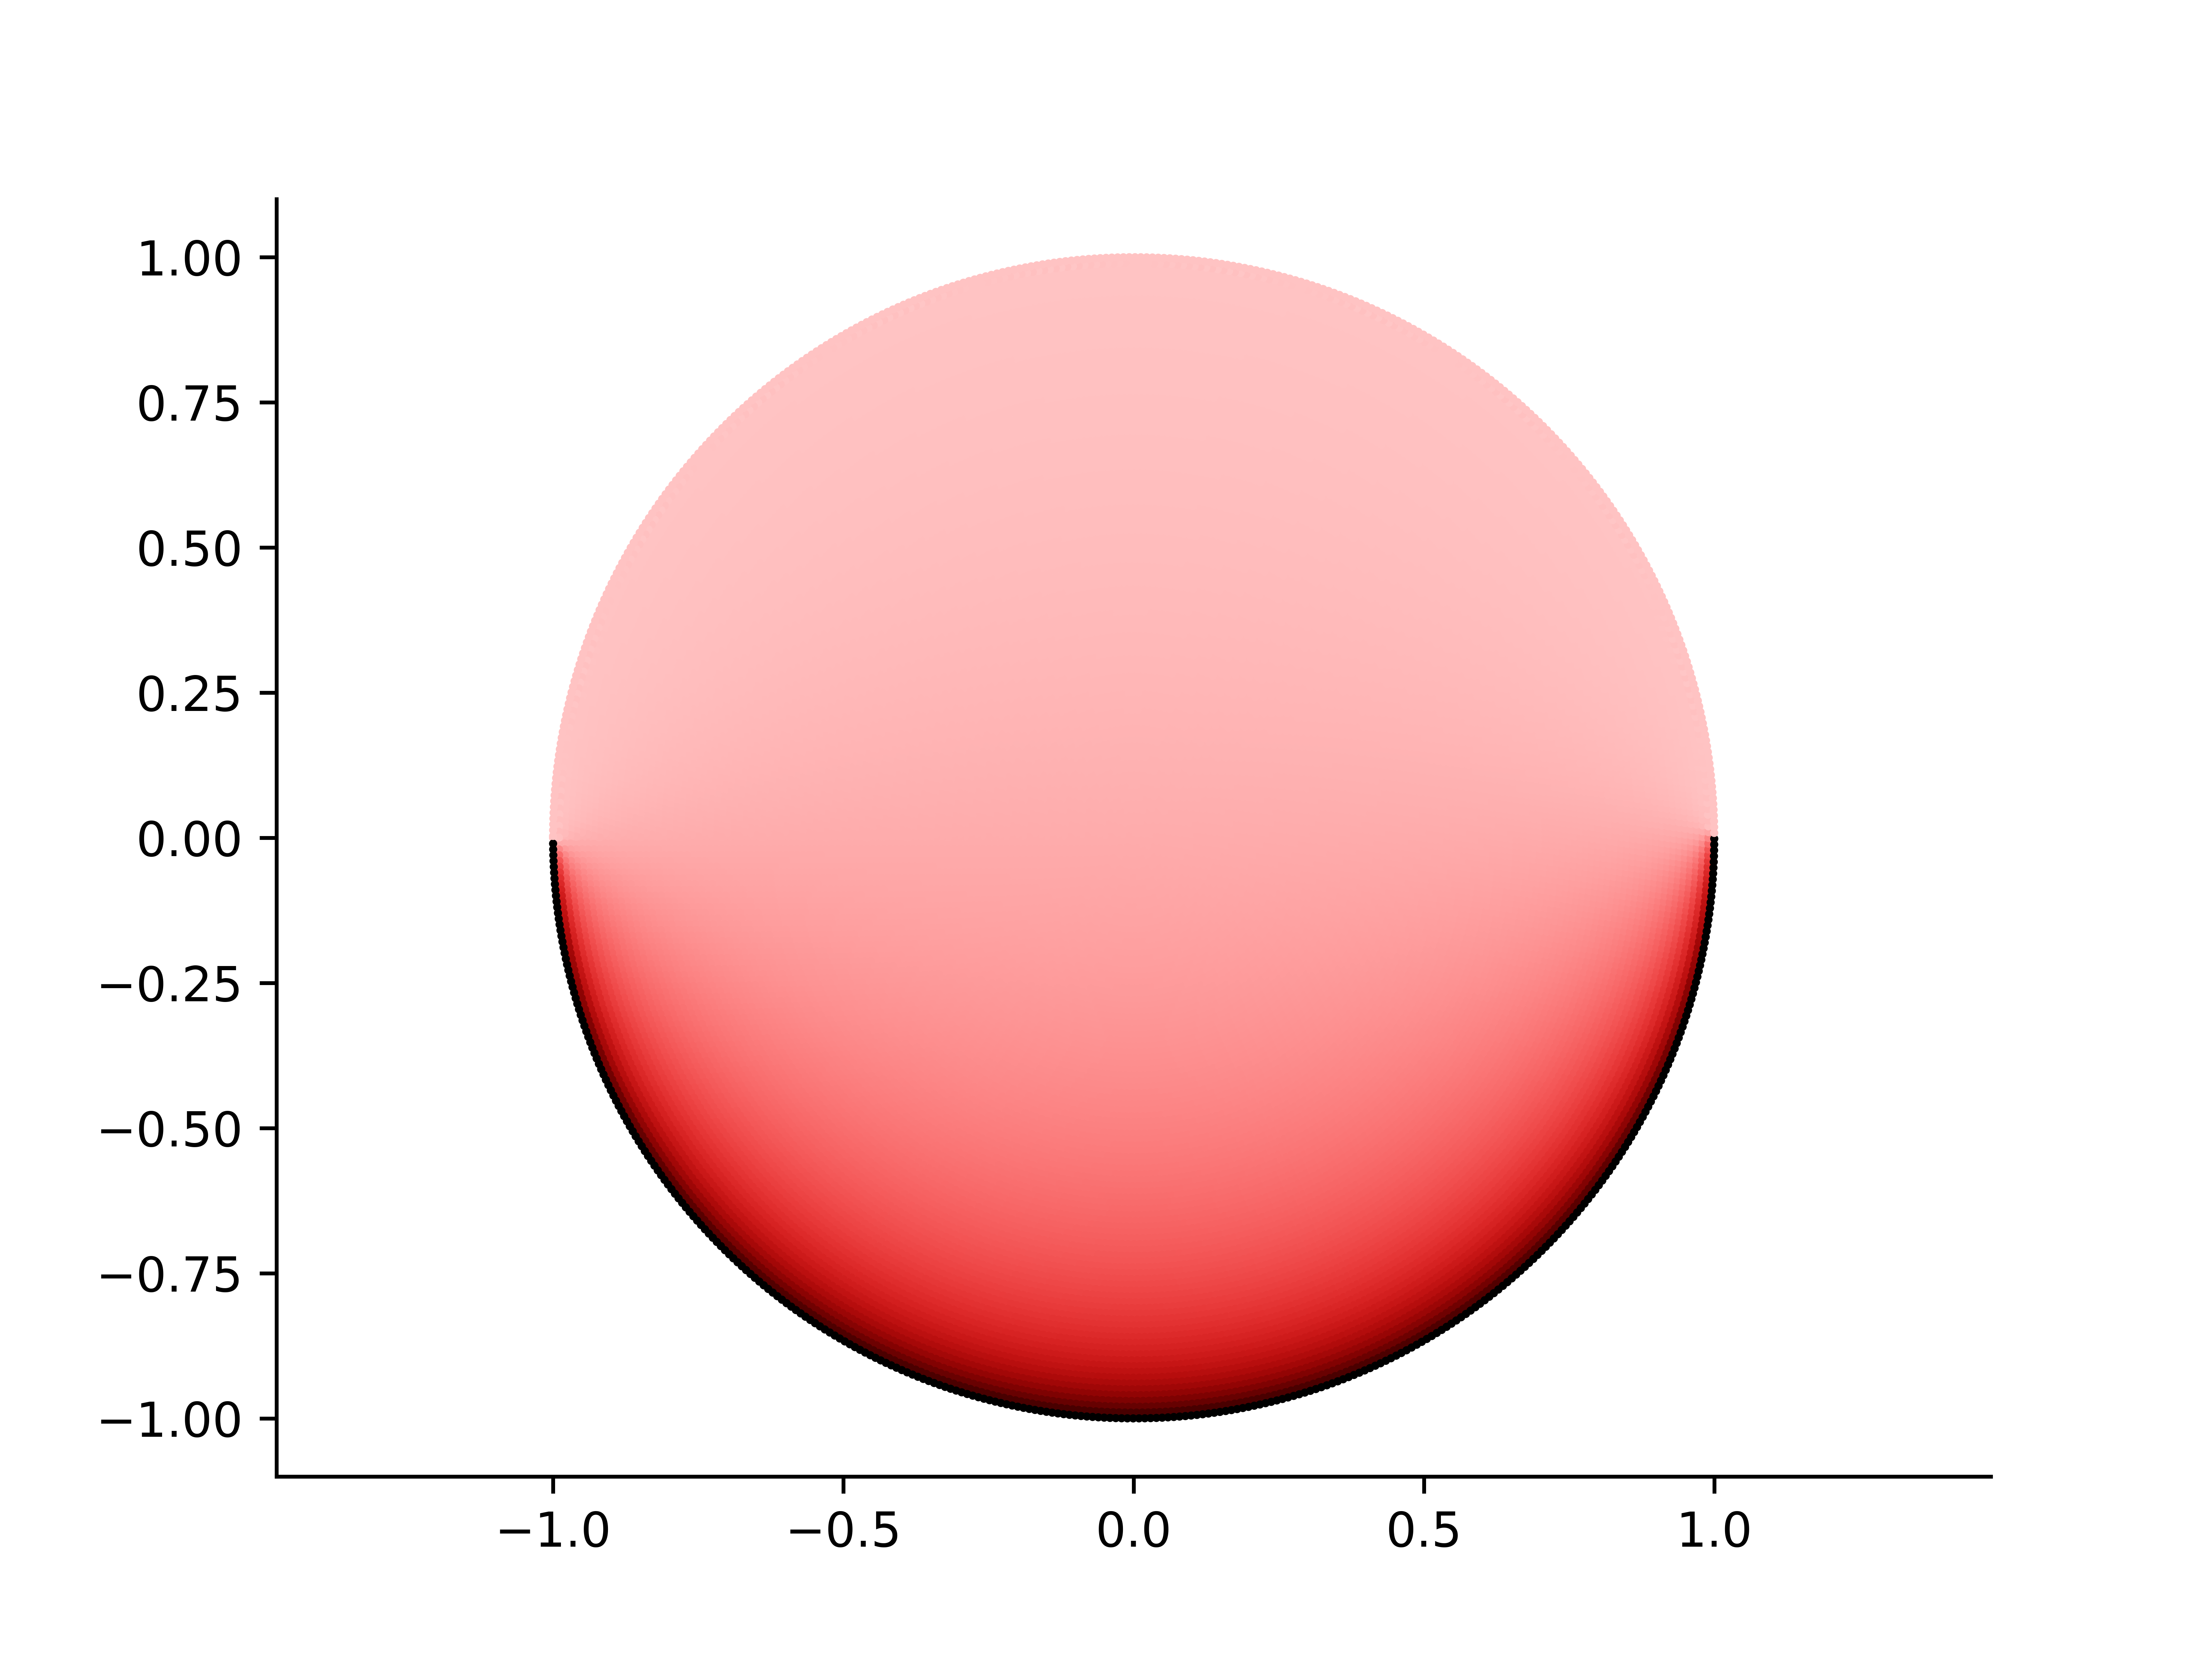
\includegraphics[width=0.49\textwidth]{../Aplicacion/atrozos.png}
    \hfil
    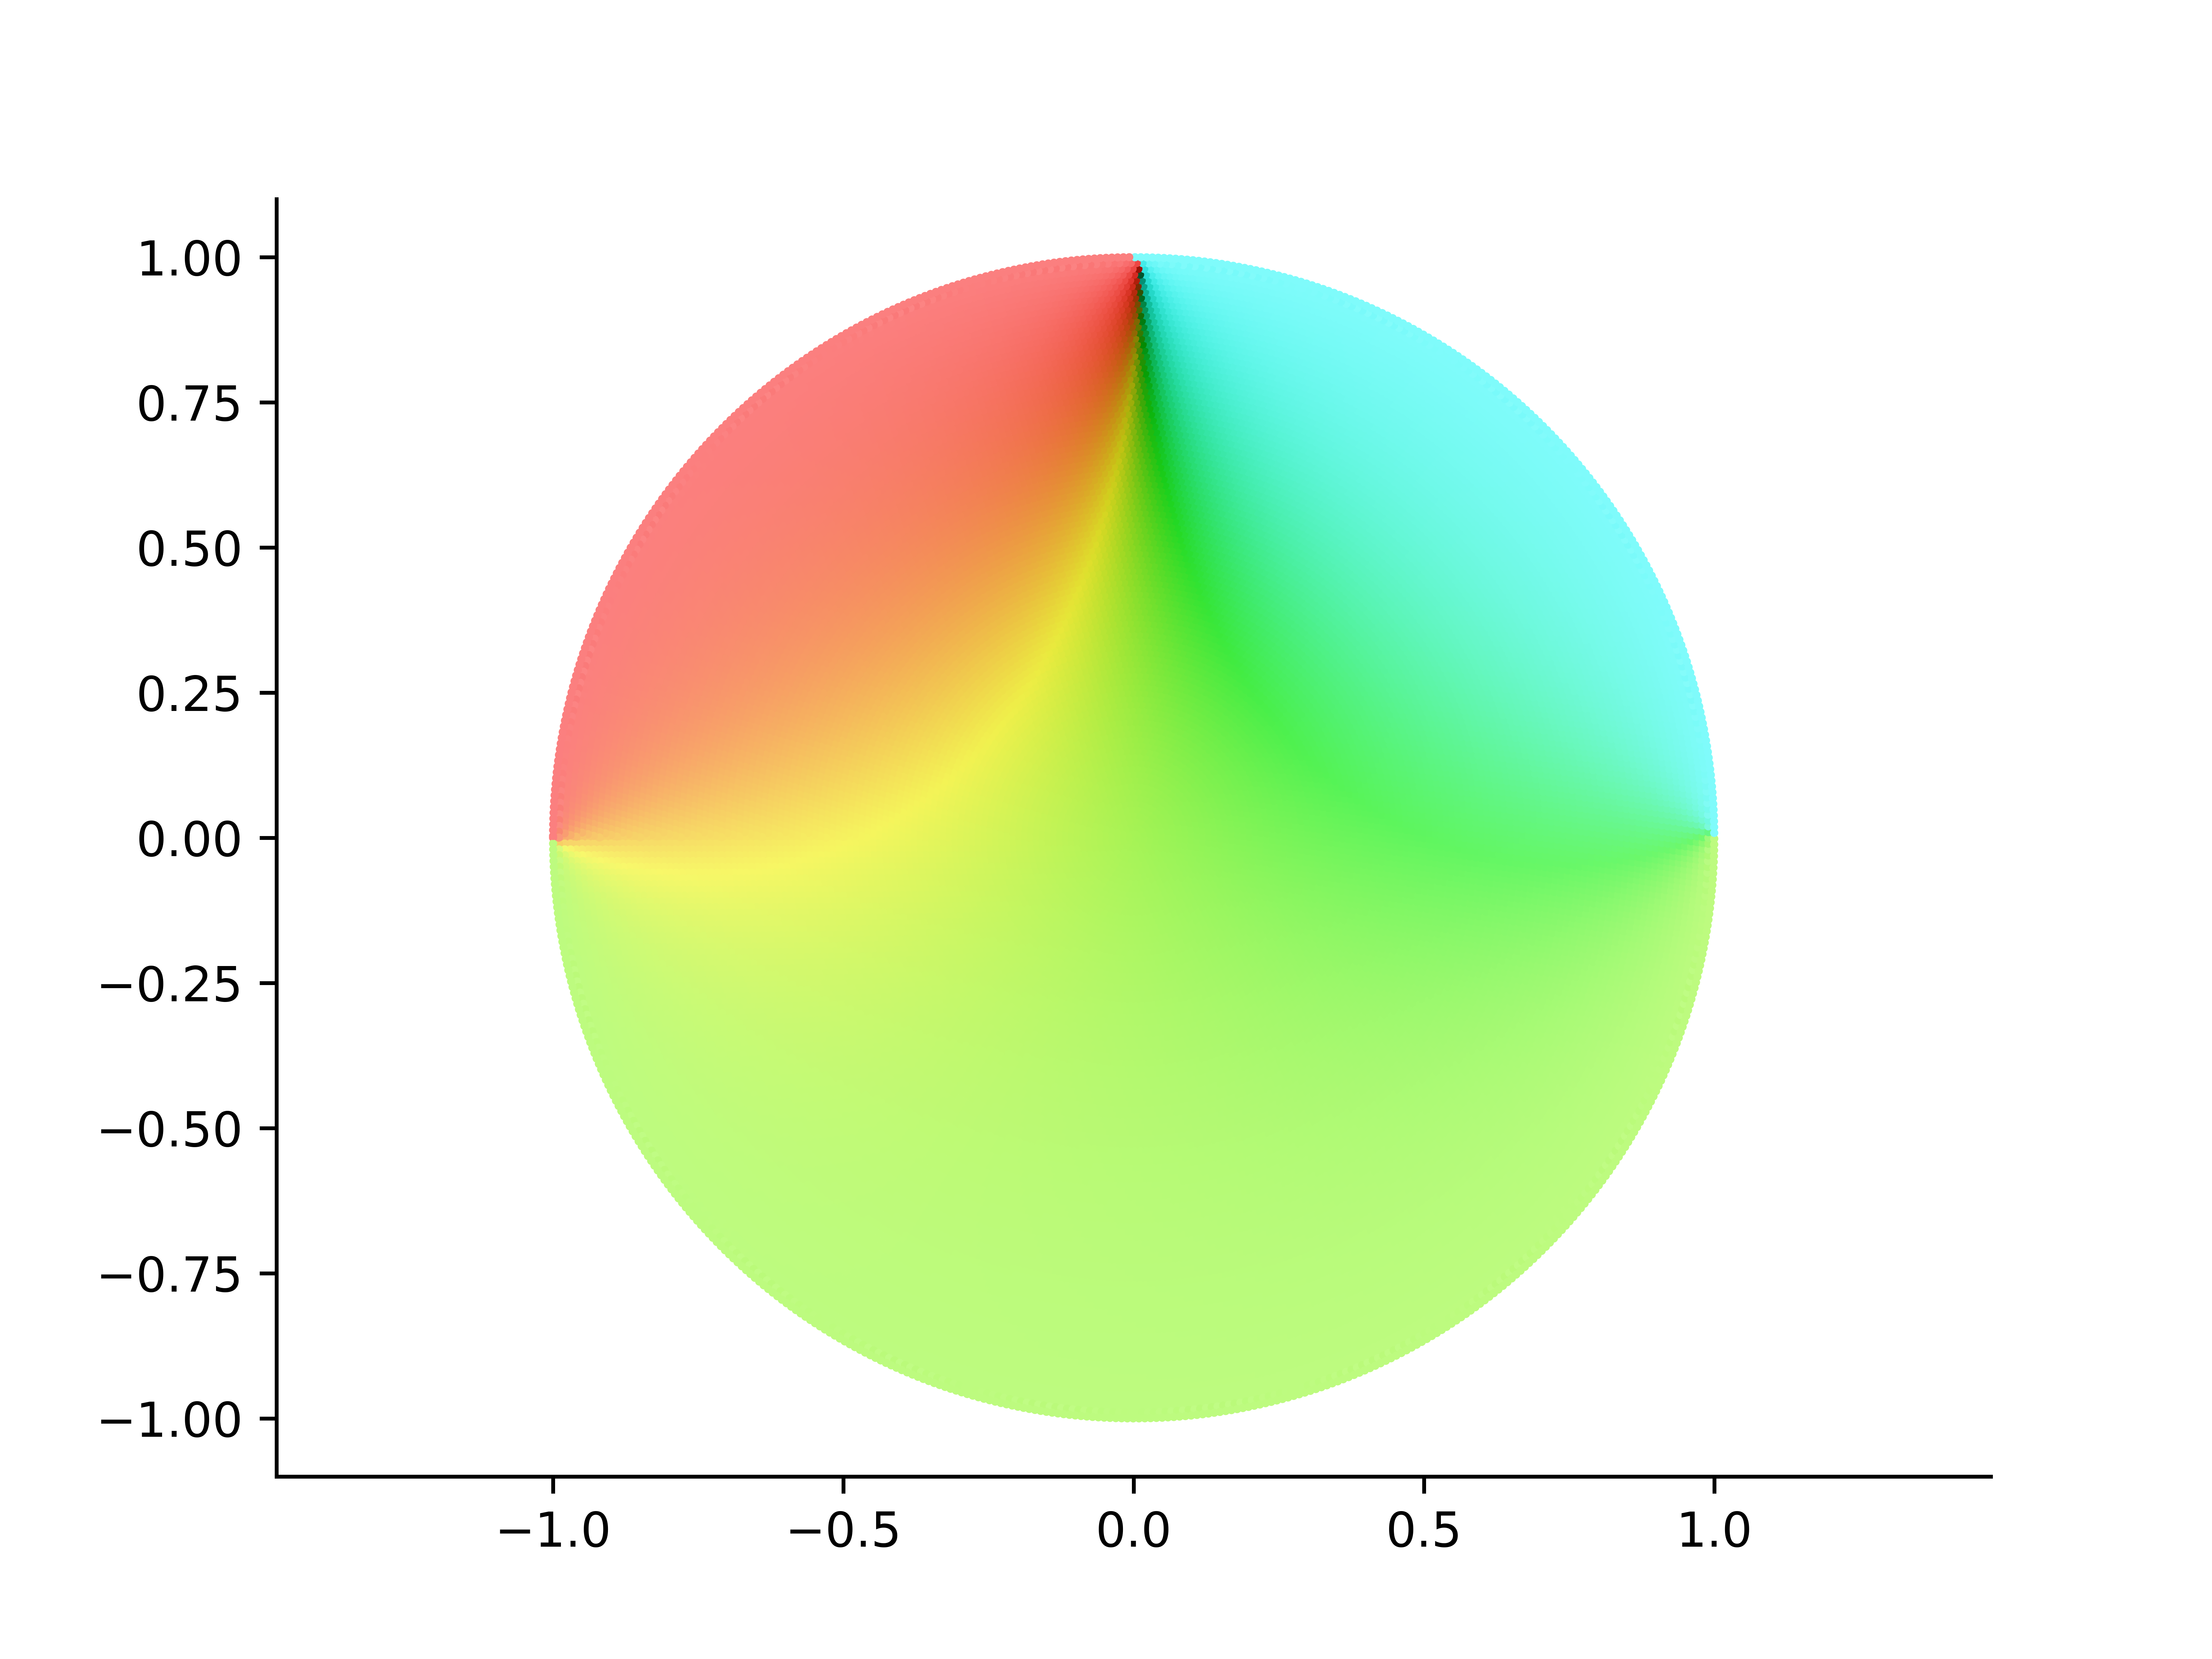
\includegraphics[width=0.49\textwidth]{../Aplicacion/atrozos(2).png}
    \caption{Funciones definidas a trozos.}
    \label{fig:atrozos}
\end{figure}

